\documentclass[times, utf8, zavrsni, square]{fer}
\usepackage{booktabs}
\usepackage{pdfpages}
\usepackage{subfig}
\usepackage{placeins}
\graphicspath{ {.} }
\setcitestyle{numbers}

\begin{document}

% TODO: Navedite broj rada.
\thesisnumber{5461}

% TODO: Navedite naslov rada.
\title{Usporedba brzine pristupa velikoj količini podataka smještenih u lokalnom datotečnom sustavu i udaljenoj radnoj memoriji}

% TODO: Navedite vaše ime i prezime.
\author{Ivan Đerek}

\maketitle

% Ispis stranice s napomenom o umetanju izvornika rada. Uklonite naredbu \izvornik ako želite izbaciti tu stranicu.
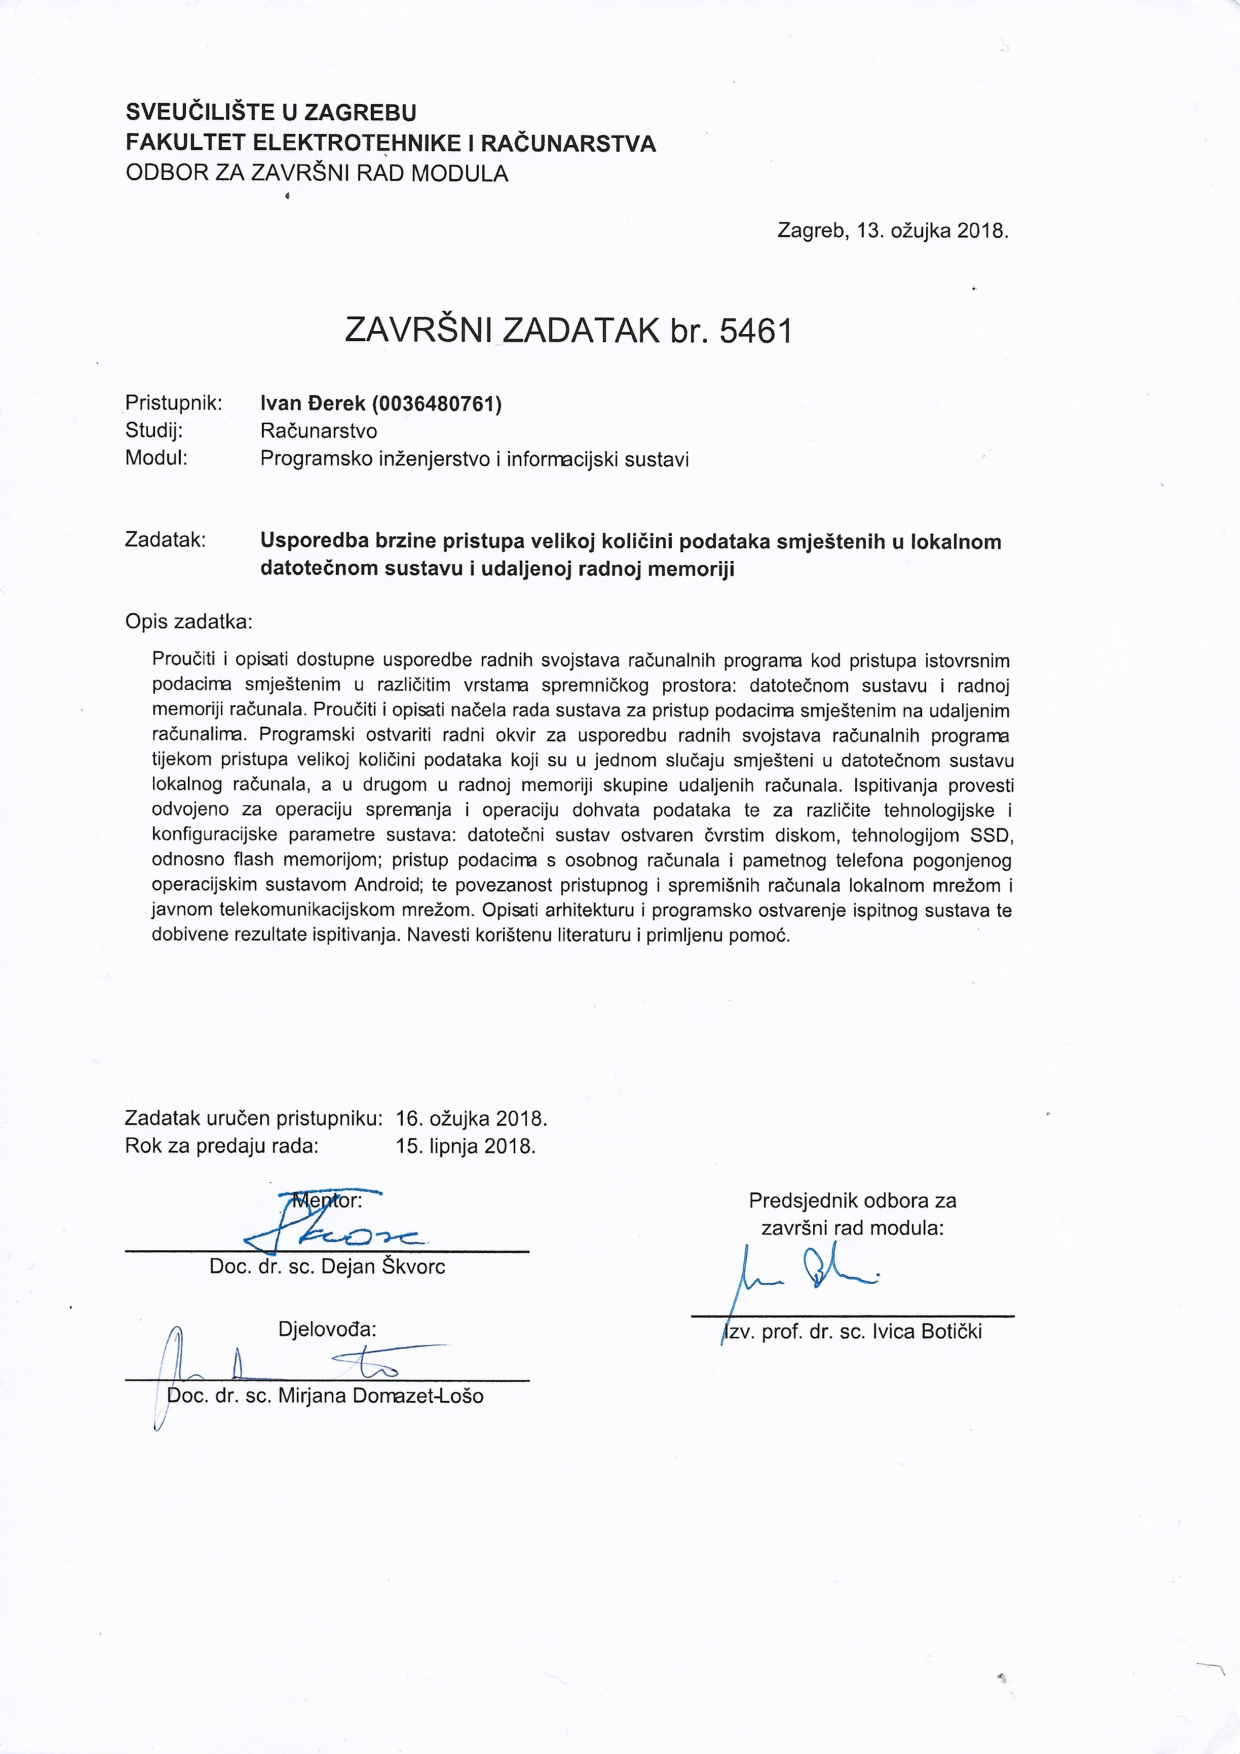
\includepdf[pages=-]{zadatak.pdf}


% Dodavanje zahvale ili prazne stranice. Ako ne želite dodati zahvalu, naredbu ostavite radi prazne stranice.
\zahvala{}

\tableofcontents

\chapter{Uvod}
Radna memorija računala najbrža je memorija na računalu, ali je skupa i nije prigodna za trajno čuvanje podataka.
Zbog toga računala imaju relativno ograničenu radnu memoriju u usporedbi s trajnom memorijom. 
Kod upravljanja većim količinama podataka može se dogoditi da radna memorija nije dovoljna pa je dio podataka potrebno držati na nekom drugom mediju,
najčešće je to trajna memorija računala. 
Drugi pristup je koristiti radnu memoriju udaljenog računala i kako bi povećali ukupni kapacitet memorije. 
Cilj ovog rada je utvrditi mogu li se pristupanjem radnoj memoriji udaljenog računala dobiti bolji rezultati nego pristupanjem lokalnom datotečnom sustavu.

U sljedećem poglavlju ovog rada predstavljaju se različiti mediji za spremanje podataka, gdje su prikazane prednosti i mane pojedinih vrsta memorija.
Nakon toga opisuje se metoda komunikacije između dvaju računala i prikazuje kako se pristupa programiranju kada je potreban sustav koji sadrži komunikaciju s udaljenim računalom.
Naposljetku je opisano programsko ostvarenje sustava za ispitivanje brzina pristupa različitim memorijama i udaljenom računalu gdje je utvrđeno kako je trajna memorija računala ipak u većini situacija brža,
ali je, uz pravi pristup, moguće brže poslati podatke na udaljeno računalo u lokalnoj mreži, nego spremiti ih na računalo.

\chapter{Mediji za spremanje podataka}
U ovom poglavlju obrađene su temeljne karakteristike različitih medija za spremanje podataka. 
Detaljnije, opisane su radna memorija (eng.\textit{ Random access Memory}, skraćeno RAM), čvrsti disk (eng.\textit{ Hard Disk Drive}, skraćeno HDD) i SSD memorija (eng.\textit{ Solid-State Drive}), te usporedba u cijeni između trajnih memorija.
\section{Radna memorija}
Radna memorija koristi se u računalima kako bi se na nju učitali programi, operativni sustav i podaci koji se trenutno koriste, kako bi im se moglo brzo pristupiti\cite{ramO}.
Radna memorija je značajno brža od trajne memorije ali zadržava podatke samo dok ima pristup napajanju, što znači da nije efikasna niti praktična za spremanje podataka na duže vrijeme\cite{ram2}.
Radna memorija je toliko brza jer se bilo kojem podatku na memoriji može pristupiti direktno, neovisno o fizičkoj lokaciji na memoriji.
Zato se uz poznatu adresu podatka na radnoj memoriji podatak može pročitati ili zapisati bez potrebe za prolaskom kroz ostale podatke, čime se značajno ubrzavaju operacija čitanja i pisanja.
To je moguće zbog arhitekture radne memorije. 
Radna memorija posložena je u stupce i redove ćelija od kojih svaka ćelija sadrži jedan bit.
Prilikom pristupanja podacima kontroler radne memorije prima adresu zapisa, nakon čega se određuju stupac i redak ćelije s koje se čita kako bi se podaci s pripadnih ćelija mogli zapisati na izlaz radne memorije.
Najbitnija karakteristika radne memorije je ta da je puno brža od trajne memorije. 
Brzina radne memorije je bitna za rad sustava jer se u nju učitavaju podaci potrebni za izvršavanje procesa na računalu.
Na slici \ref{fig:ram} prikazan je primjer kako izgleda radna memorija.
\begin{figure}[h]
    \centering
    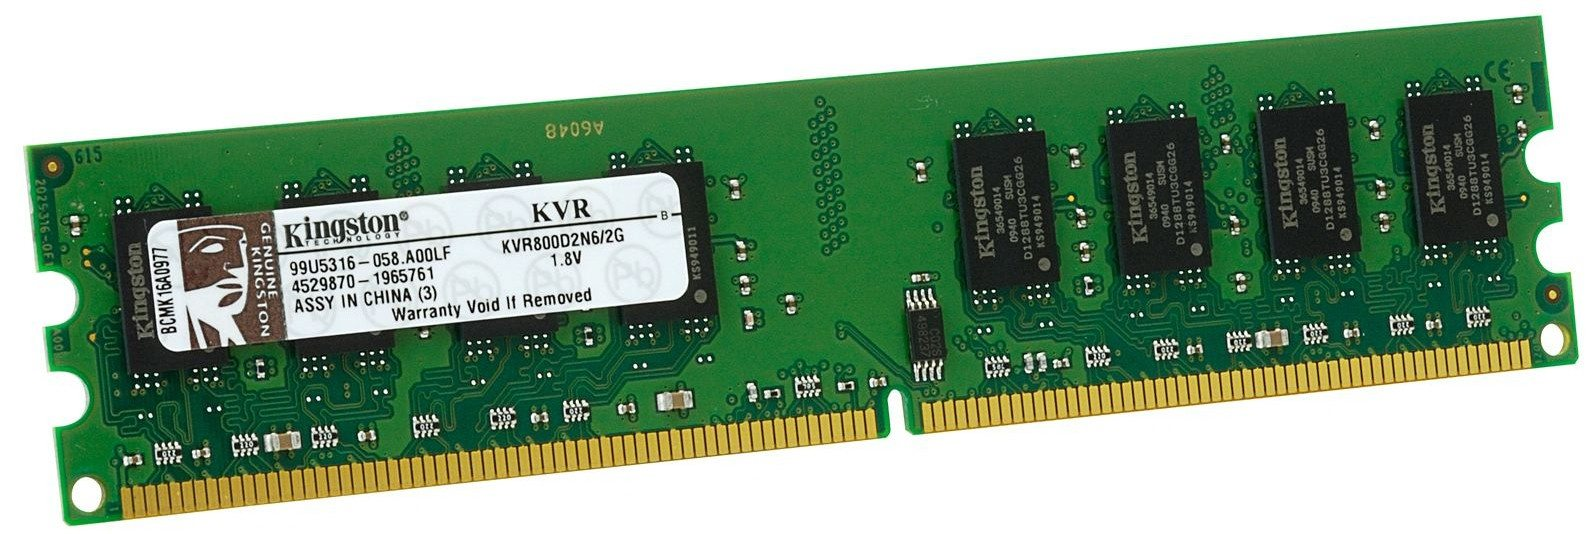
\includegraphics[width=1\textwidth]{ram}
    \caption{Radna memorija}
    \label{fig:ram}
\end{figure}
\FloatBarrier
\section{Trajna memorija}
Pod trajnu memoriju računala spada memorija koja se koristi za trajno skladištenje podataka na računalu.
Najčešće implementacije su čvrsti disk i ssd memorija.
Trajna memorija je uvijek sporija od radne memorije, ali je zato uvijek značajno većeg kapaciteta.
Ove razlike između trajne memorije i radne memorije postoje jer one nemaju istu namjenu u računalu. 
Dok se radna memorija koristi za programe i podatke koji su trenutno potrebni za izvođenje procesa, trajna memorija koristi se za skladištenje podataka između korištenja.
Kada se podaci s lokalne memorije koriste, učitavaju se u radnu memoriju kako bi pristup istim podacima bio brži i spremniji za korištenje, 
u suprotnom bi procesor morao čekati da se učita podatak s lokalne memorije i time bi se značajno usporio rad računala.
Trajnu memoriju zato koristimo ako želimo trajno spremiti podatak bez da ga izgubimo pri gašenju sustava.
Problem nastaje ako se u radnu memoriju ne mogu učitati svi potrebni podaci, u tom je slučaju potrebno dio podataka privremeno zapisati na trajnu memoriju kako bi se oslobodio prostor za nove podatke.
Budući da u toj situaciji dolazi do potrebe za češćim čitanjem i pisanjem na trajnu memoriju, brzina trajna memorije igra veliku ulogu. 
Ali nisu sve trajne memorije jednake. Čvrsti diskovi se koriste već duže vrijeme i imaju značajan kapacitet te relativno nisku  cijenu.
Novija ssd memorija u istom cjenovnom razredu ima značajno niži kapacitet, ali jednako tako i brži pristup podacima.
\subsection{Čvrsti disk}
Čvrsti disk\cite{hdd} magnetni je disk podijeljen u male površine koje mogu individualno biti magnetizirane ili demagnetizirane.
Na taj način se spremaju bitovi podataka koji ostaju zapisani čak i bez napajanja.
Na slici \ref{fig:hddImage} prikazan je primjer takvog diska.
Čitanje i pisanje podataka s diska obavlja se pomoću magnetske glave koja se može pomicati između centra i ruba čvrstog diska.
Svim dijelovima diska može se pristupiti jer se disk konstantno okreće dok je aktivan.
Jedan od razloga zašto je čitanje i pisanje s čvrstog diska sporije je taj što da bi se pristupilo podacima, 
glava se mora fizički pomaknuti te disk okrenuti na pravu lokaciju, vrijeme potrebno da se nađe podatak zove se vrijeme traženja.
Vrijeme traženja ovisi o brzini vrtnje diska, vremenu da se magnetska glava pomakne na točnu lokaciju i načinu zapisivanja ili čitanja podataka\cite{hdd2}.
Osim što takav mehanički pristup uzrokuje sporije čitanje i zapis podataka, on utječe i na pouzdanost ovog medija.
Kako ima puno pokretnih dijelova može se dogoditi da se neki od dijelova mehanički ošteti i tada se više ne može pristupiti podacima na disku.
Unatoč tim manama čvrsti diskovi su i dalje popularni oblik spremanja podataka, uglavnom zbog cijene i duge tradicije korištenja.

\begin{figure}[h!]
    \centering
    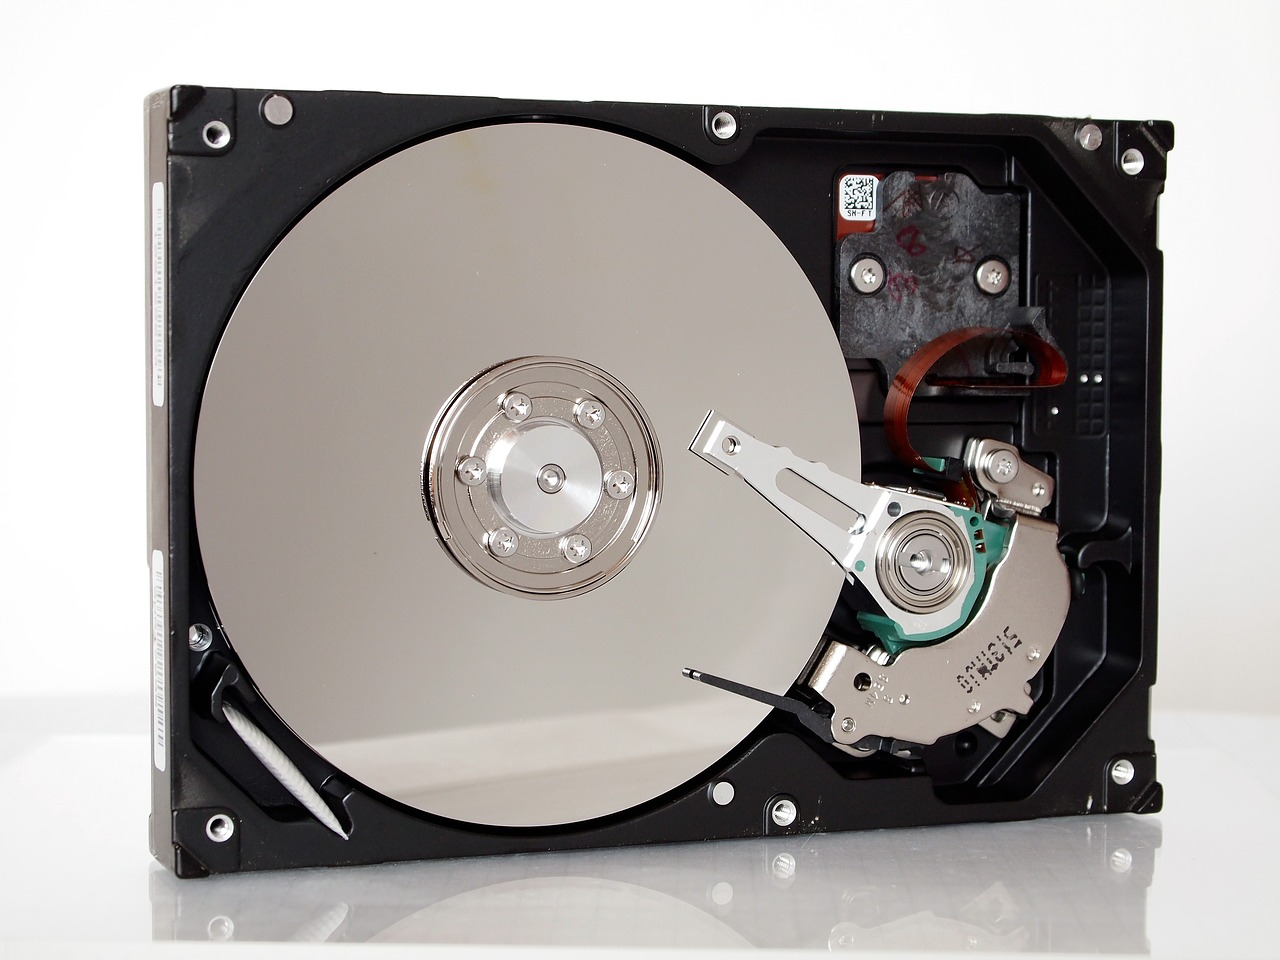
\includegraphics[width=1\textwidth]{hdd}
    \caption{Primjer čvrstog diska}
    \label{fig:hddImage}
\end{figure} 
\FloatBarrier
\subsection{SSD memorija}
SSD memorija koristi nili (eng. \textit{NAND})\footnote{(\textit{not and}) logički sklop koji obavlja operaciju suprotnu od operacije i (eng. \textit{AND})} logičke sklopove implementirane tranzistorima kako bi trajno spremila podatke. 
Ta vrsta memorije ponekad se još zove i brza memorija (eng. \textit{flash memory}) zbog toga što je brža u odnosu na čvrsti disk.
Za razliku od radne memorije, tranzistori na SSD memoriji zadržavaju informaciju čak i kada nisu pod napajanjem, zbog čega se takva memorija može koristiti za lokalni datotečni sustav. 
Budući da ova memorija nema pokretne dijelove, podacima je moguće pristupiti puno brže nego na čvrstom disku jer im se, poput kod radne memorije, može pristupiti direktno.
Dodatna prednost manjka pokretnih dijelova je ta što se time smanjuje mogućnost mehaničkog oštećenja, a time se dobiva i na stabilnosti memorije.
Tranzistori u takvoj memoriji omogućuju zapis podataka pomoću različitih razina napona, koji se neće promijeniti kada se ukine dovod struje do diska\cite{ssd}.
Naravno, osim što je takva memorija sporija od radne memorije, i dalje  se podaci moraju najprije učitati na radnu memoriju kako bi ih koristili.
Danas SSD memorija postaje sve popularnija i već je standardno da računala imaju SSD memoriju barem kao glavnu memoriju, time osiguravaju brže učitavanje operativnog sustava računala i brži rad aplikacija koje se spremaju na glavnu memoriju.
\begin{figure}[h!]
    \centering
    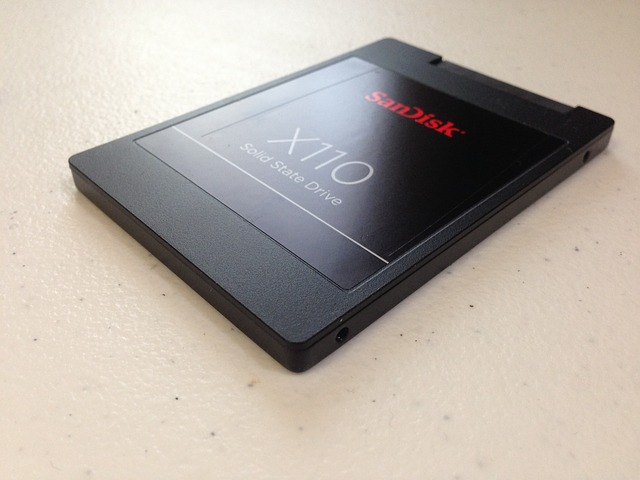
\includegraphics[width=1\textwidth]{ssd}
    \caption{Primjer SSD memorije}
    \label{fig:ssdImage}
\end{figure} 
\FloatBarrier
\subsection{Cjenovna usporedba SSD memorije i čvrstog diska}
Iako je ustanovljeno da je SSD memorija puno brža i pouzdanija, čvrsti diskovi su i dalje prisutni na tržištu.
Glavni razlog tome je cijena. Danas je popularno imati SSD kao glavnu memoriju i uz njega sporedni čvrsti disk visokog kapaciteta.
Time se postižu optimalne performanse sustava i istovremeno zadovoljavaju sve veće potrebe za velikim kapacitetom memorije.
Najbolji način za usporedbu cijena je usporedba cijene po gigabajtu na memoriji. 
Tablica \ref{fig:prices} prikazuje cijenu nekih čvrstih diskova u randima\footnote{Službena valuta Južnoafričke Republike}.
Može se vidjeti kako je kod čvrstih diskova cijena po gigabajtu najniža pri 4TB, dok je kod SSD memorije pri 1TB i tu je razlika u cijeni po gigabajtu skoro 10 puta veća\cite{prices}, dok se za cijenu čvrstog diska od 8TB može kupiti SSD memorija od najviše 1TB.
Iz toga je lako zaključiti zašto se čvrsti diskovi i dalje koriste u tako velikom broju.
\begin{figure}[h!]
    \centering
    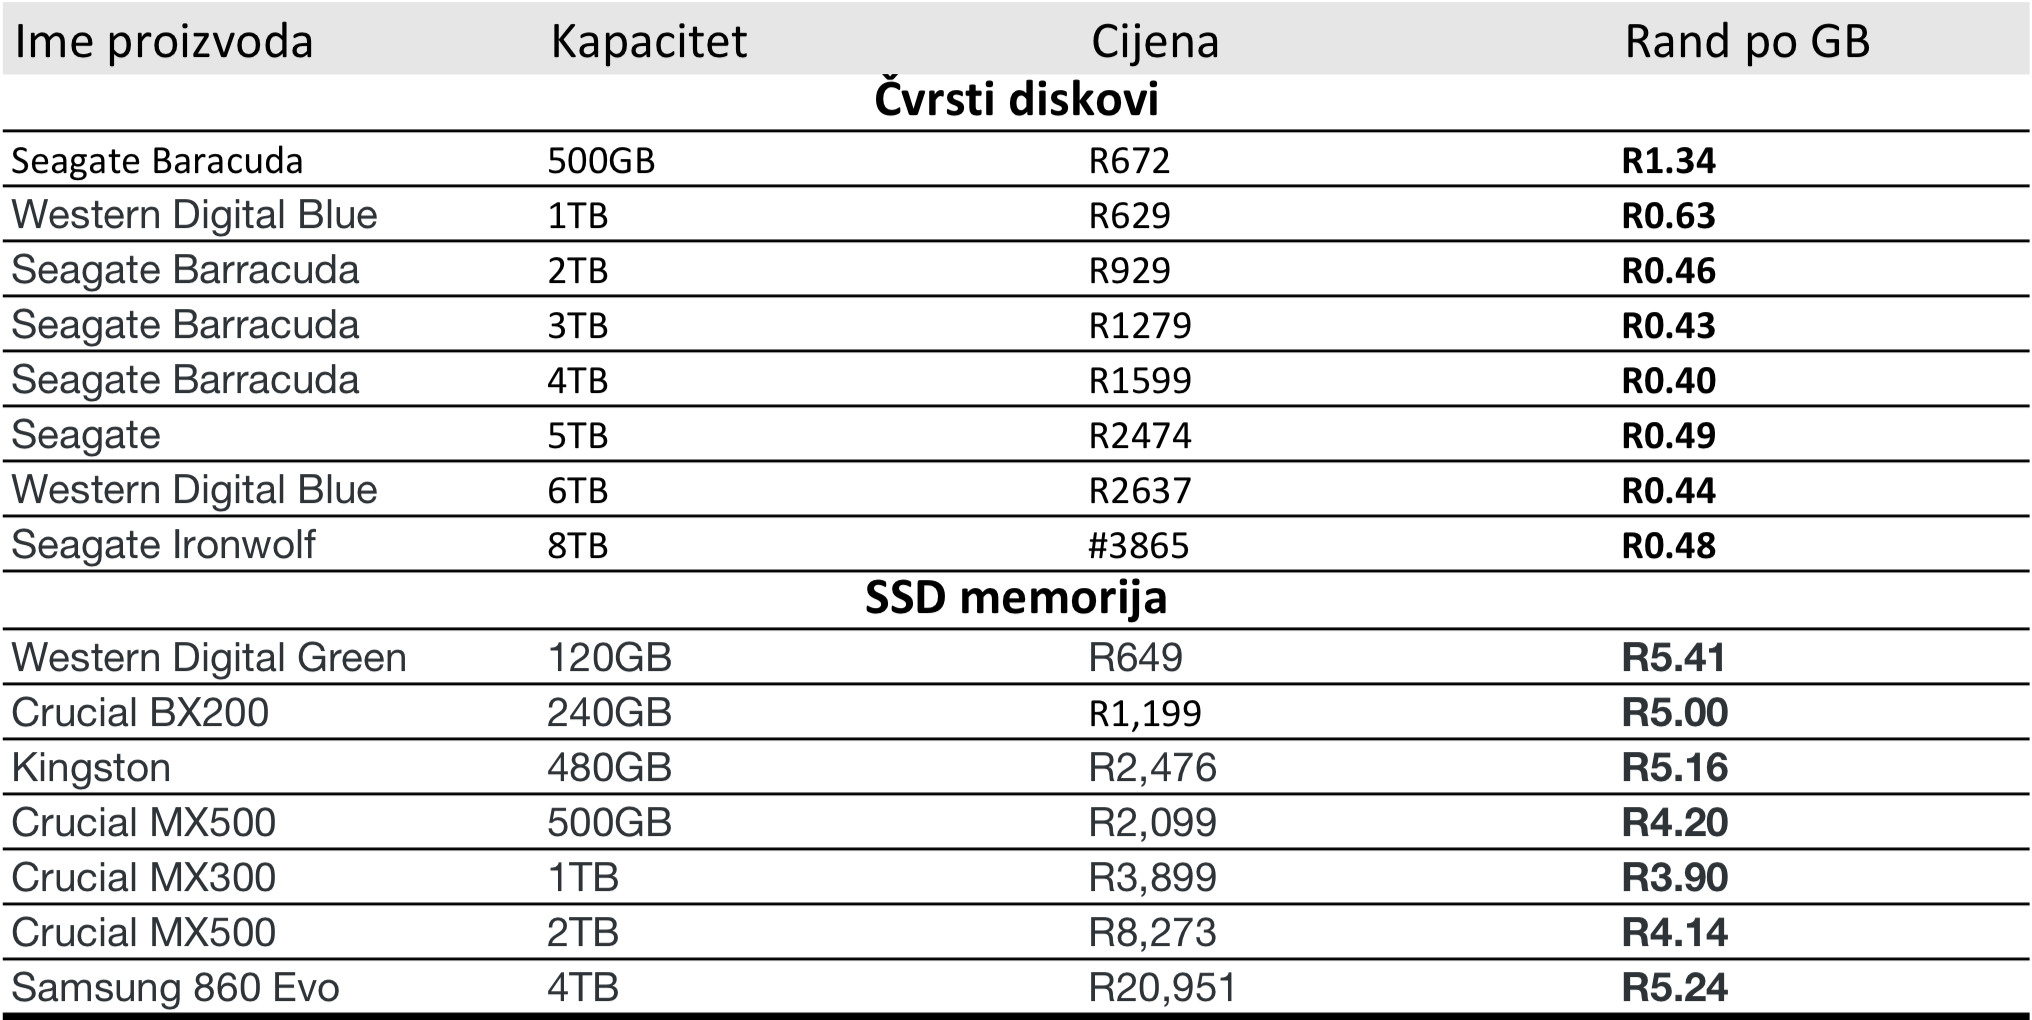
\includegraphics[width=1\textwidth]{memory_prices}
    \caption{Tablica s primjerima cijena memorija}
    \label{fig:prices}
\end{figure} 
\FloatBarrier
\chapter{Komunikacija računalnom mrežom}
U moderno vrijeme sve su popularnija različita rješenja poput spremanja podataka u "oblaku" (eng. \textit{Cloud storage})\footnote{Popularan naziv za skladištenje podataka na mreži kako bi im se moglo pristupiti s raznih lokacija.} i korištenja resursa s udaljenih računala.
Razlog tome je što je prijenos podataka putem javne mreže sve brži i praktičniji za korištenje.
Jednom kada su podaci na udaljenom računalu, mogu se spremiti na bilo koji od oblika trajne memorije ili na radnu memoriju tog računala.
Najbrže se može pristupiti podacima koji se nalaze na radnoj memoriji udaljenog računala, odnosno oni podaci koji su već spremni za prijenos putem mreže.
Ako je moguće pouzdano pristupati tim podacima onda je izmjena podataka podacima slična kao s trajnom memorijom.
Naime kako bi se podaci koristili moraju se nalaziti na radnoj memoriji računala. Ako je tih podataka previše za radnu memoriju računala mora ih se spremiti na neku drugu memoriju.
Uobičajeno rješenje je spremiti ih na lokalnu trajnu memoriju, ali ako se ti podaci nalaze u radnoj memoriji drugog računala postoje određene prednosti.
Kada bi prijenos podataka preko mreže bio brži nego učitavanje s trajne memorije onda bi prednost bila očita, moguće bi bilo koristiti radnu memoriju računala na mreži koja se trenutno ne koristi i upotrijebiti je kao brzu memoriju za računalo na kojem je potrebna.
Čak i ako je prijenos podataka sporiji činjenica je da bi se na udaljenom računalu ti podaci već nalazili u radnoj memoriji i
moguće je obaviti dio posla paralelno na tom udaljenom računalu, time bi se ubrzao ukupan posao tako da se na kraju dohvati samo rezultat operacija.
Zadnja velika prednost ovakvog rješenja je ta što, ako se omogući pristup podacima s udaljenog računala, njima se može pristupiti s više računala i lokacija.
\FloatBarrier
\pagebreak
\section{Mrežna priključna točka}
Mrežna priključna točka (eng. \textit{Network socket}) programsko je sučelje pruženo \linebreak
TCP (eng. \textit{Transmission Control Protocol})\footnote{internet protokol kod kojeg se pazi da je poruka primljena} 
ili UDP (eng. \textit{User Datagram\linebreak Protocol}) protokolom\cite{socket}.
To je priključna točka za komunikaciju s udaljenim\linebreak računalom definirana IP (eng. \textit{Internet protocol}) adresom i pristupnom točkom (eng. \textit{port})\footnote{identifikacija procesa ili mrežne usluge na računalu}.
Razlog iz kojeg je potrebna pristupna točka je taj što mrežna priključna točka ne predstavlja cijelo računalo nego samo proces koji je otvoren za komunikaciju. 
IP adresa određuje samo uređaj, a na njemu se može obavijati više procesa, 
kako bi se moglo spojiti na ispravan proces potrebna nam je pristupna točka\cite{socket2}.
\begin{figure}[h!]
    \centering
    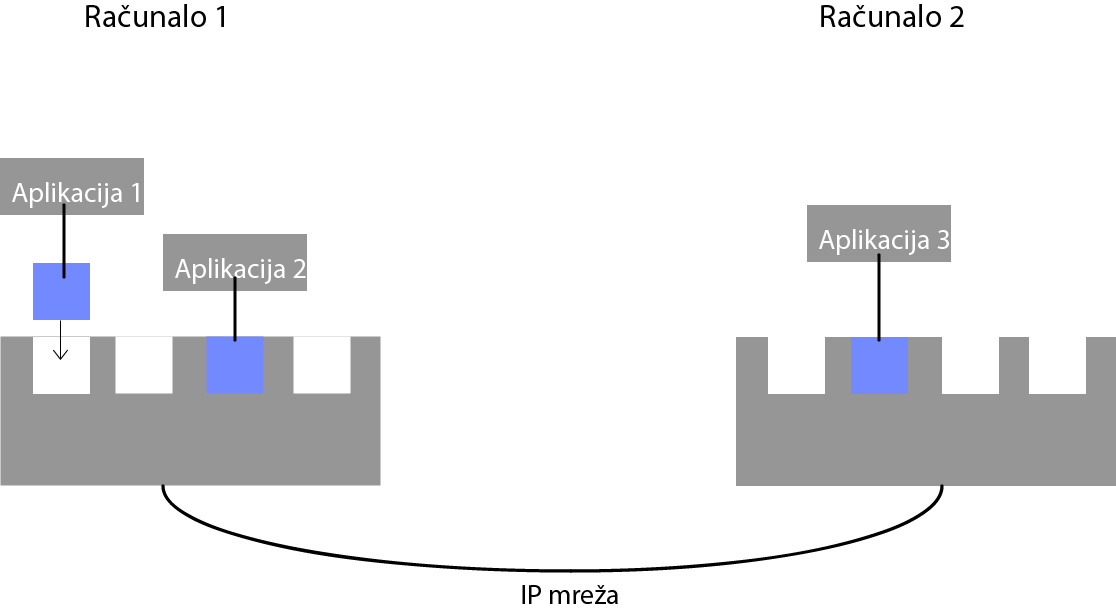
\includegraphics[width=1\textwidth]{sockets}
    \caption{Mrežne priključne točke omogućuju komunikaciju između aplikacija na udaljenim računalima}
    \label{fig:sockets}
\end{figure} 
Ako je bitno da podaci ostanu u prvobitnom stanju koristi se povezanost pomoću TCP/IP servisa.
Naime iako je bitna brzina prijenosa podataka, ono što je bitnije je da se ti podaci cjelovito prenesu, inače mogu izgubiti svoju korisnost.
Kod programiranja s priključnim točkama jedan proces je u ulozi poslužitelja, dok je drugi klijent, glavna razlika među njima je pri uspostavljanju veze, naime klijent mora znati IP adresu i pristupnu točku poslužitelja kako bi se spojio, nakon što je veza uspostavljena komunikacija je obostrana i poslužitelj i klijent su ravnopravni.
Mrežna priključna točka može obavljati sljedeće 4 osnovne operacije: spajanje s udaljenom priključnom točkom, slanje podataka, primanje podataka i zatvaranje veze.
Kod takve komunikacije potrebno je prvo spojiti dva računala, što se započinje otvaranjem veze na poslužitelju.
Kako bi se klijent spojio na poslužitelj, prvo mora znati IP adresu računala na kojem je poslužitelj i pristupnu točku procesa koji je u ulozi poslužitelja.
Veza se zatim inicira sa strane klijenta koji se pokušava spojiti na poznatu IP adresu i pristupnu točku.
Jednom kad je veza potvrđena može se započeti slanje podataka.
Podaci se šalju putem izlaznih i ulaznih sljedova podataka (eng. \textit{stream}) mrežnih priključnih točaka.

\FloatBarrier
\section{Programiranje s mrežnim priključnim točkama}
Moguće je koristiti više različitih implementacija na bazi mrežnih priključnih točaka, ali kod svih je jednako to da sadrže osnovne operacije.
U Java programskom jeziku koriste se java.net.Socket i java.net.ServerSocket klase\cite{oracle}.
Najbitnije metode ServerSocket klase:

\begin{enumerate}
    \itemsep0em
    \item accept(), vraća Socket, osluškuje vezu na mrežnoj priključnoj točki i prihvaća ju
    \item bind(SocketAddress endpoint), vraća void, veže mrežnu priključnu točku na zadanu adresu koja se sastoji od IP adrese i pristupne točke
    \item close(), vraća void, zatvara mrežnu priključnu točku
    \end{enumerate}

ServerSocket na sebe veže IP adresu i pristupnu točku koja mu se zada te počinje osluškivati vezu metodom accept().
Jednom kada ServerSocket primi zahtjev za spajanjem, prihvaća ga i time dobiva referencu na mrežnu priključnu točku kako bi se mogli otvoriti sljedovi podataka(eng. \textit{data stream}) između priključnih točaka.
Najbitnije metode Socket klase su:


\begin{enumerate}
    \itemsep0em
    \item connect(SocketAddress endpoint), vraća void, veže mrežnu priključnu točku na poslužitelja koji se nalazi na zadanoj IP adresi i pristupnoj točki
    \item bind(SocketAddress endpoint), vraća void, veže mrežnu priključnu točku na zadanu adresu koja se sastoji od IP adrese i pristupne točke
    \item getInputStream(), vraća InputStream, InputStream nam je potreban za čitanje podataka koje prima mrežna pristupna točka
    \item getOutputStream(), vraća OutputStream, OutputStream nam je potreban za slanje podataka na povezanu mrežnu pristupnu točku
    \item close(), vraća void, zatvara mrežnu priključnu točku
    \end{enumerate}

Na klijentskoj aplikaciji potrebno je znati IP adresu i pristupnu točku na koji je vezan ServerSocket kako bi se iniciralo spajanje.
Jednom kada je veza uspostavljena, klijent i poslužitelj mogu komunicirati.
Komunikacija se obavlja putem sljedova podataka na priključnim točkama.
Svaka strana ima svoj ulazni i izlazni slijed podataka koji je spojen na priključnu točku drugog procesa.
Dalje se programira upravljanjem sljedova podataka.
Primjer jednostavnih aplikacija poslužitelja i klijenta može se vidjeti na slikama \ref{fig:server_example} i \ref{fig:client_example}.


\begin{figure}[h!]
    \centering
    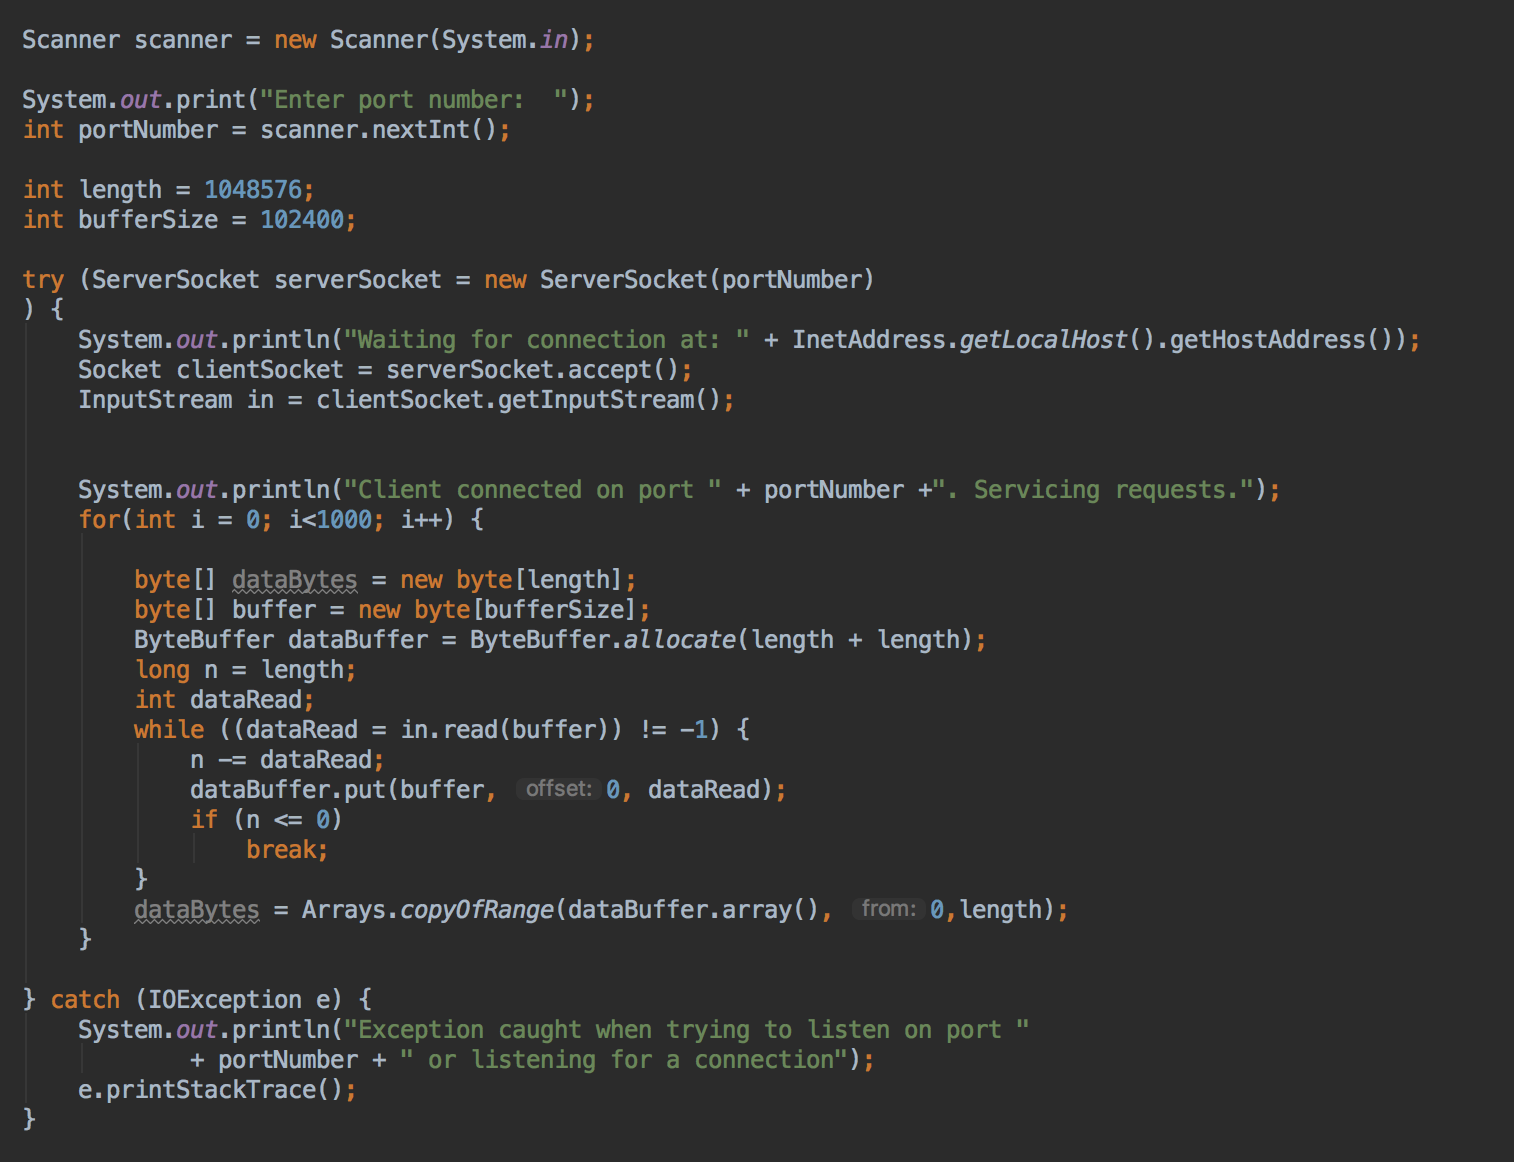
\includegraphics[width=1\textwidth]{server_example}
    \caption{Isječak jednostavne poslužiteljske aplikacije}
    \label{fig:server_example}
\end{figure} 
\begin{figure}[h!]
    \centering
    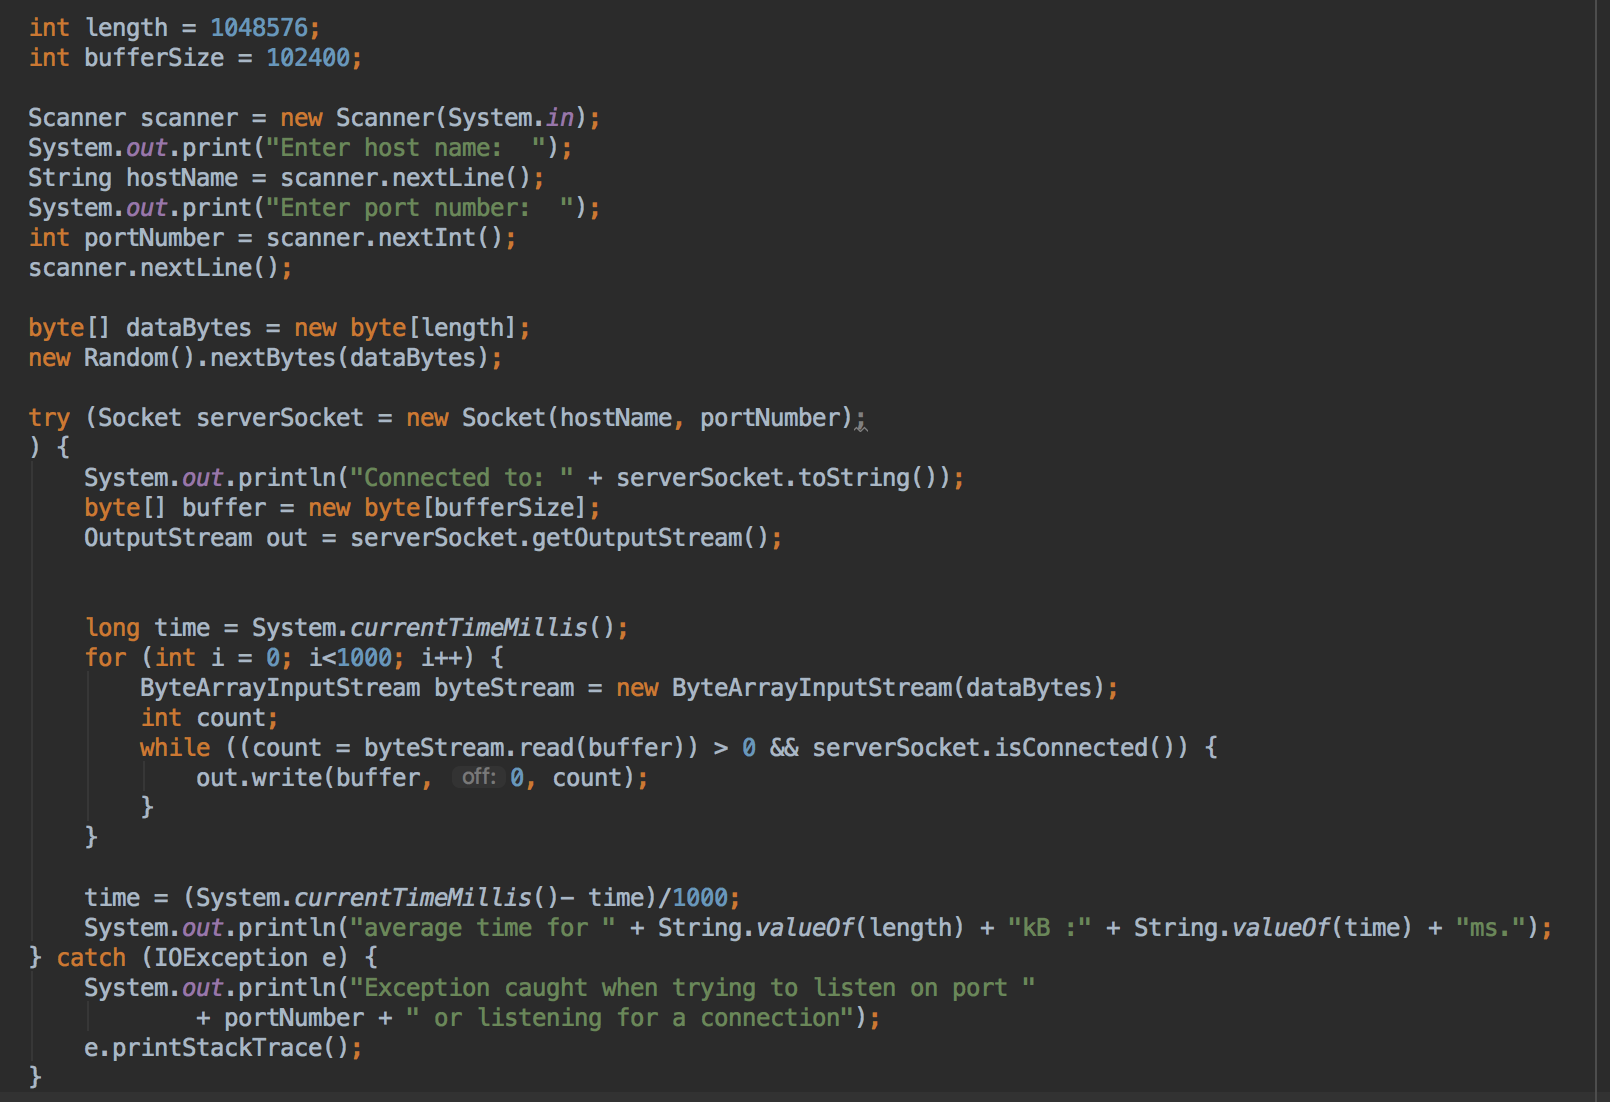
\includegraphics[width=1\textwidth]{client_example}
    \caption{Isječak jednostavne klijentske aplikacije}
    \label{fig:client_example}
\end{figure} 
\FloatBarrier
\chapter{Programsko ostvarenje i rezultati sustava za ispitivanje}
Za potrebe istraživanja za ovaj rad bilo je potrebno napraviti jednostavnu aplikaciju koja ima pristup radnoj memoriji na udaljenom računalu.
Aplikacija mora spremati i čitati podatke s udaljenog računala i lokalne memorije te zabilježiti vremena pisanja i čitanja podataka kako bi se moglo usporediti razlike u brzini pristupa podacima na različitim memorijama.
Aplikacija je rađena u Java programskom jeziku koristeći IntelliJ Idea razvojno okruženje za računalne aplikacije i C\# programskom jeziku u sustavu Xamarin koristeći Visual Studio razvojno okruženje za Android aplikaciju.

Osnovna ideja sustava koji testira brzine prijenosa podataka je da se zabilježi vrijeme prije prijenosa podataka, 
obavi prijenos i onda odredi koliko je vremena prošlo. 
Budući da prijenos ne traje svaki put jednako, za precizniju informaciju potrebno je izračunati prosjek vremena trajanja iz puno ponovljenih prijenosa s istim podacima.
Radi toga se u klijentu koji radi testiranje, prijenos podataka ponavlja i na kraju se ukupno vrijeme dijeli s brojem prijenosa, kao kod primjera pisanja podataka na poslužitelj koji je prikazan na slici \ref{fig:time}. 
U sklopu istraživanja provodi se više različitih testova. 
Na slici \ref{fig:relations} prikazani si odnosi klijentskih aplikacija s poslužiteljem. Za svaku prikazanu liniju mogu se obaviti operacije pisanja i čitanja.

\begin{figure}[h!]
    \centering
    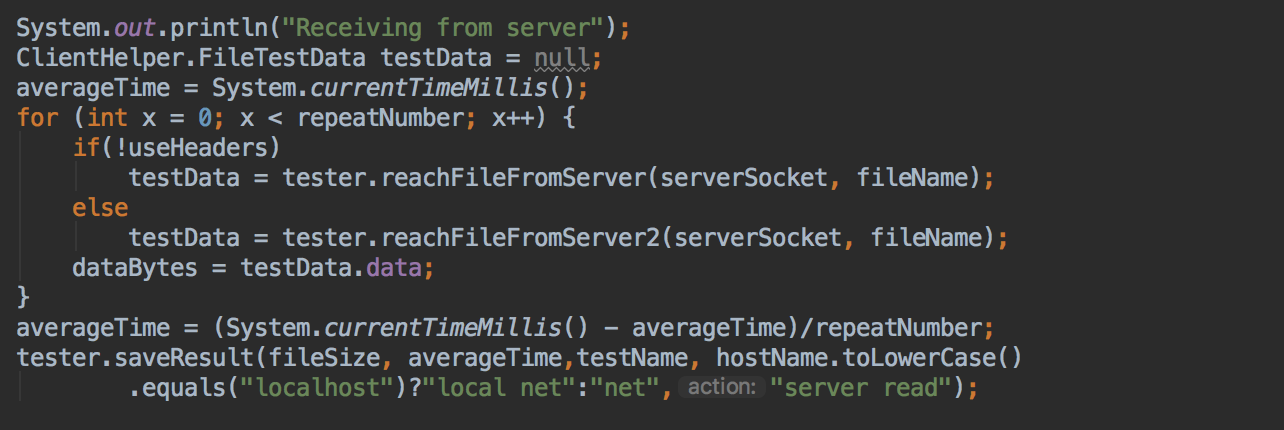
\includegraphics[width=1\textwidth]{time_measure}
    \caption{Isječak koda za testiranje brzine slanja podataka na poslužitelj koristeći veći broj uzastopnih testova}
    \label{fig:time}
\end{figure} 
\begin{figure}[h!]
    \centering
    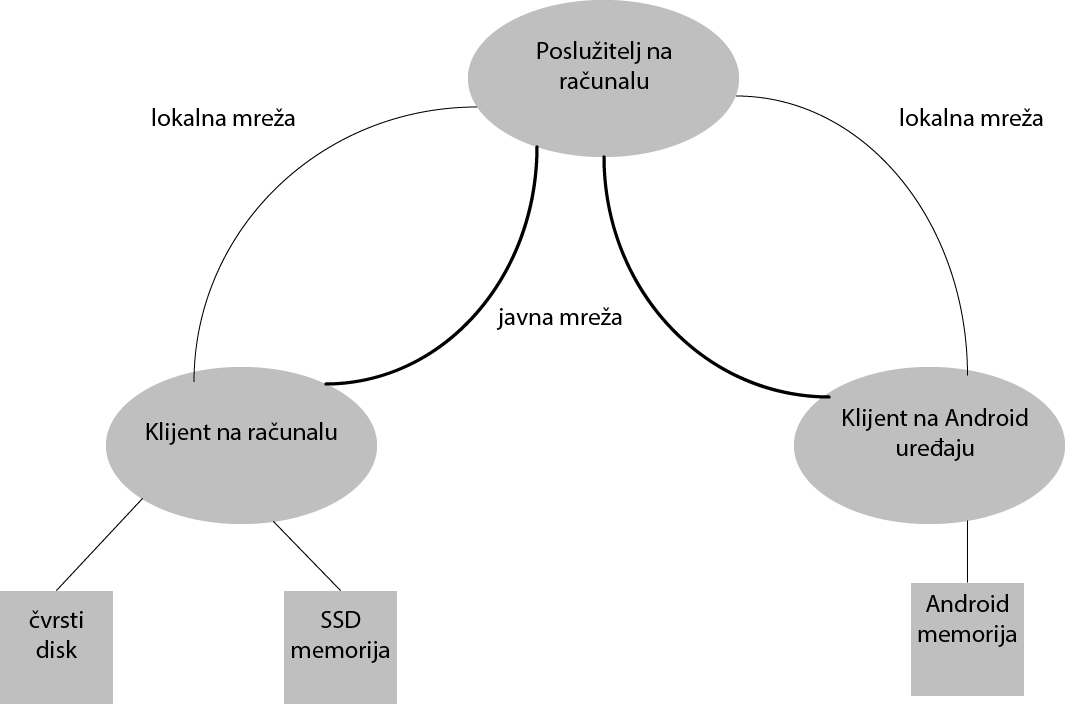
\includegraphics[width=1\textwidth]{graf_relations}
    \caption{Prikaz odnosa među aplikacijama i njihovih pripadnih memorija}
    \label{fig:relations}
\end{figure} 

Aplikacija za računalo napisana u Java programskom jeziku sastoji se od tri klase: Server, AutoClient i ClientHelper. 
Klase koje se mogu pokrenuti su Server i AutoClient dok ClientHelper opisuje metode korištenja podataka na klijentu.
AutoClient i Client se razlikuju u tome što je za AutoClient potrebno unijeti samo osnovne podatke i dalje generira veliki broj testova, dok Client traži korisnika da stalno unosi naredbe.
Aplikacije su napisane kao jednostavne aplikacije za terminal.
Server ima dva objekta koji predstavljaju mrežne priključne točke, jedan predstavlja priključnu točku na poslužitelju, dok drugi predstavlja priključnu točku na klijentu.
Prvo je potrebno stvoriti mrežnu priključnu točku na poslužitelju i dodijeliti mu pristupnu točku, nakon čega se čeka da klijent započne spajanje.
Kada se klijent spoji poslužitelj dobiva informacije o klijentu kako bi mogao koristiti ulazne i izlazne sljedove podataka povezane s klijentom.
Dalje poslužitelj prima informaciju o načinu na koji će razmjenjivati podatke (putem više poruka ili pomoću zaglavlja koja nose više informacija) i zatim ponavlja petlju u kojoj od klijenta prima poruku s informacijom o naredbi koju radnju klijent želi obaviti.
Svaki klijent ima samo referencu na mrežnu pristupnu točku od poslužitelja. 
Metode za pisanje i čitanje s trajne memorije mogu se vidjeti na slici \ref{fig:memory_pc}.


\begin{figure}[h!]
    \centering
    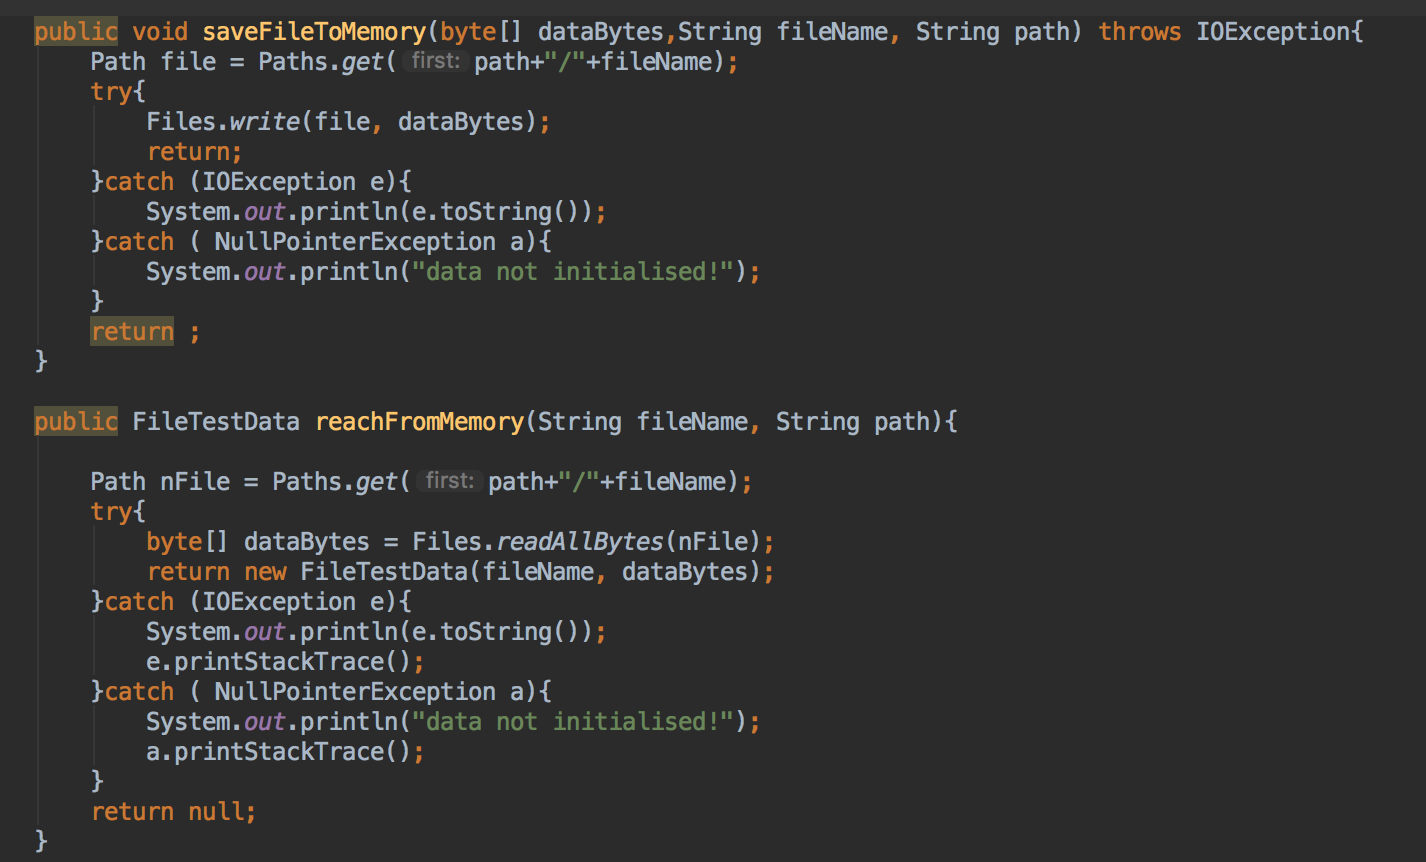
\includegraphics[width=1\textwidth]{memory_pc}
    \caption{Isječak koda za pisanje i čitanje podataka s trajne memorije računala}
    \label{fig:memory_pc}
\end{figure}

Aplikacija za android uređaje napisana u C\# programskom jeziku sastoji se od\linebreak jednog zaslona i pomoćne klase koja upravlja komunikacijom s poslužiteljem. 
Android aplikacija ne može se koristiti kao poslužitelj, nego se ponaša jednako kao AutoClient u aplikaciji na računalu.
Aplikacija sadržava ClientHelper klasu koja je jednaka kao ona na računalu, samo prepisana u C\#, zato se klijent na mobilnom uređaju ponaša jednako kao onaj na računalu u komunikaciji s poslužiteljem.
Jedina razlika u ClientHelper klasi na android aplikaciji je u pristupu trajnoj memoriji zbog specifičnosti android operativnog sustava, primjer se može vidjeti na slici \ref{fig:memory_andr}.
Sučelje aplikacije sastoji se od polja za upis IP adrese računala, polja za upis pristupne točke, gumba za pokretanje testova i prikaza na kojem se vide informacije o testiranju u tijeku.
\begin{figure}[h!]
    \centering
    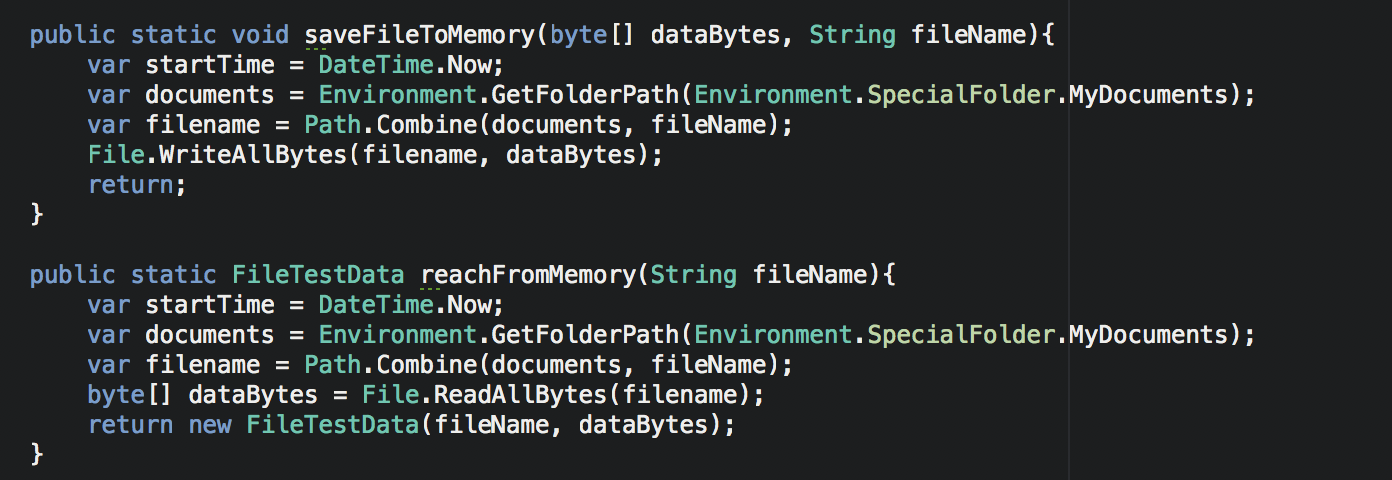
\includegraphics[width=1\textwidth]{memory_andr}
    \caption{Isječak koda za pisanje i čitanje podataka s trajne memorije Android uređaja}
    \label{fig:memory_andr}
\end{figure}

\FloatBarrier
\section{Sustav sa strogim potvrđivanjem}

Kako bi poslužitelj znao koju radnju treba obaviti moramo mu najprije poslati poruku sa sljedećom radnjom. 
Prvotna ideja je da se svaka poruka šalje zasebno te zatim čekaju potvrde od poslužitelja da je informacija primljena kako bi se nastavilo s radom.
Protok komunikacije može se vidjeti na slici \ref{fig:graf_1}.
Nakon slanja informacija potrebnih za čitanje podatka, podaci se šalju u dijelovima kako se ne bi preopteretio slijed podataka.
Poslužitelj primljene podatke sprema u listu te koristi odvojenu listu naziva podataka s odgovarajućim indeksima.
Ako poslužitelj primi podatak naziva koji već ima, prebrisat će se stari podatak.
Veličina podataka koja se odjednom šalje je najviše pola MB\footnote{mebi bajt}, naime ako se šalju pre veliki podaci od jednom, sustav često zapne u komunikaciji.
Za svaku radnju na kraju se zapisuje rezultat koji sadrži:

    \begin{enumerate}
    \itemsep0em
    \item vrijeme izvršavanja testa
    \item vrstu testa (slanje ili primanje podataka na poslužitelj ili lokalnu memoriju)
    \item veličinu podataka u KiB
    \item proteklo vrijeme između početka i kraja zapisivanja ili čitanja podataka u ms
    \item medij na kojem se zapisao ili nalazio podatak (mreža, čvrsti disk ili ssd memorija)
    \item ime testa
    \end{enumerate}

    \begin{figure}[t]
        \centering
        \subfloat[zapis podataka]{{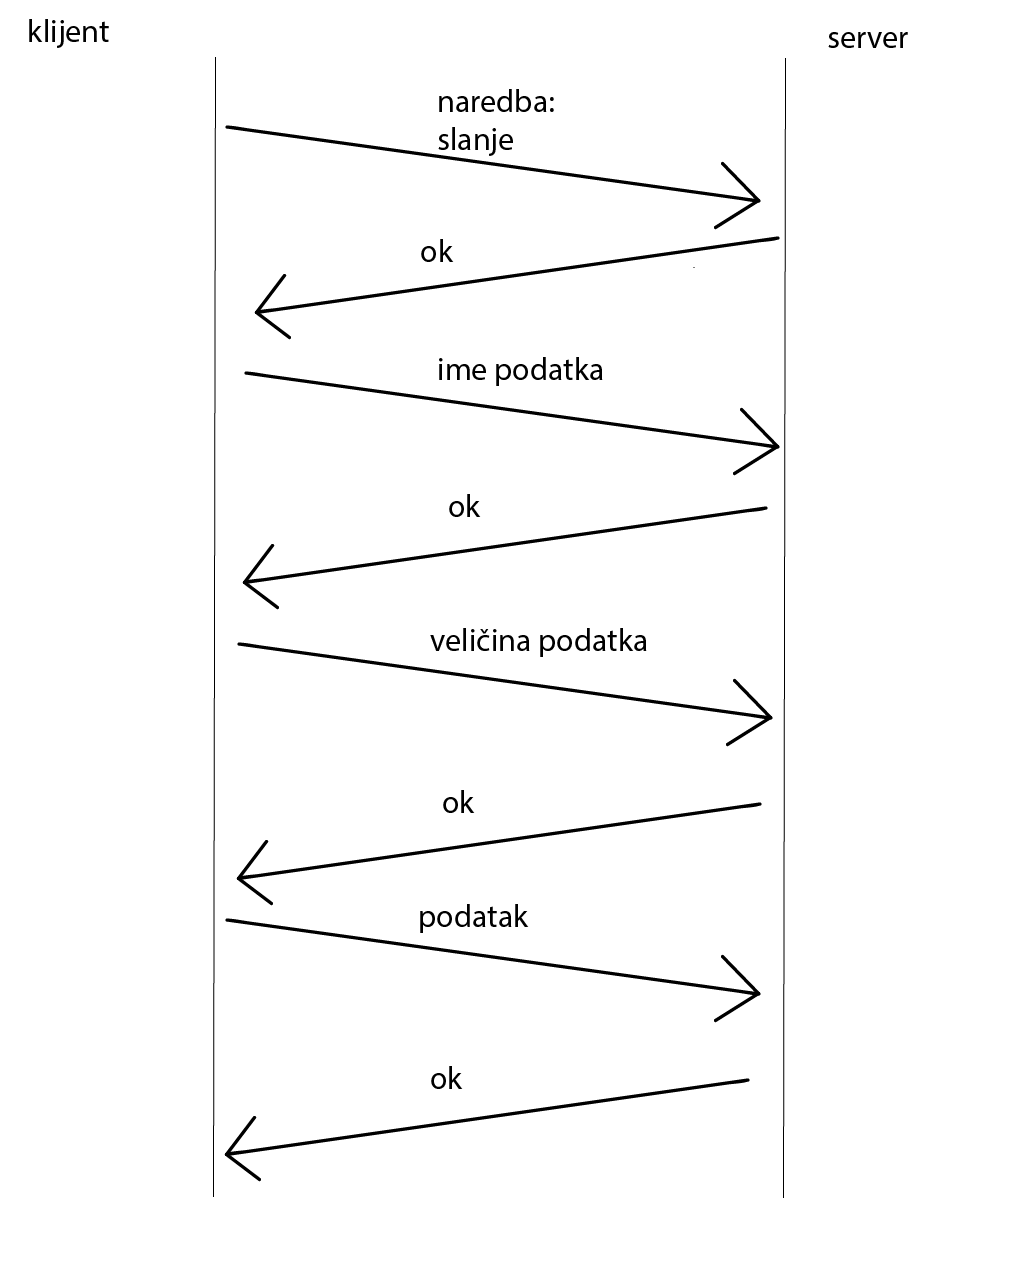
\includegraphics[width=0.5\textwidth]{graf_slanje_1}}}%
        \centering
        \subfloat[čitanje podataka]{{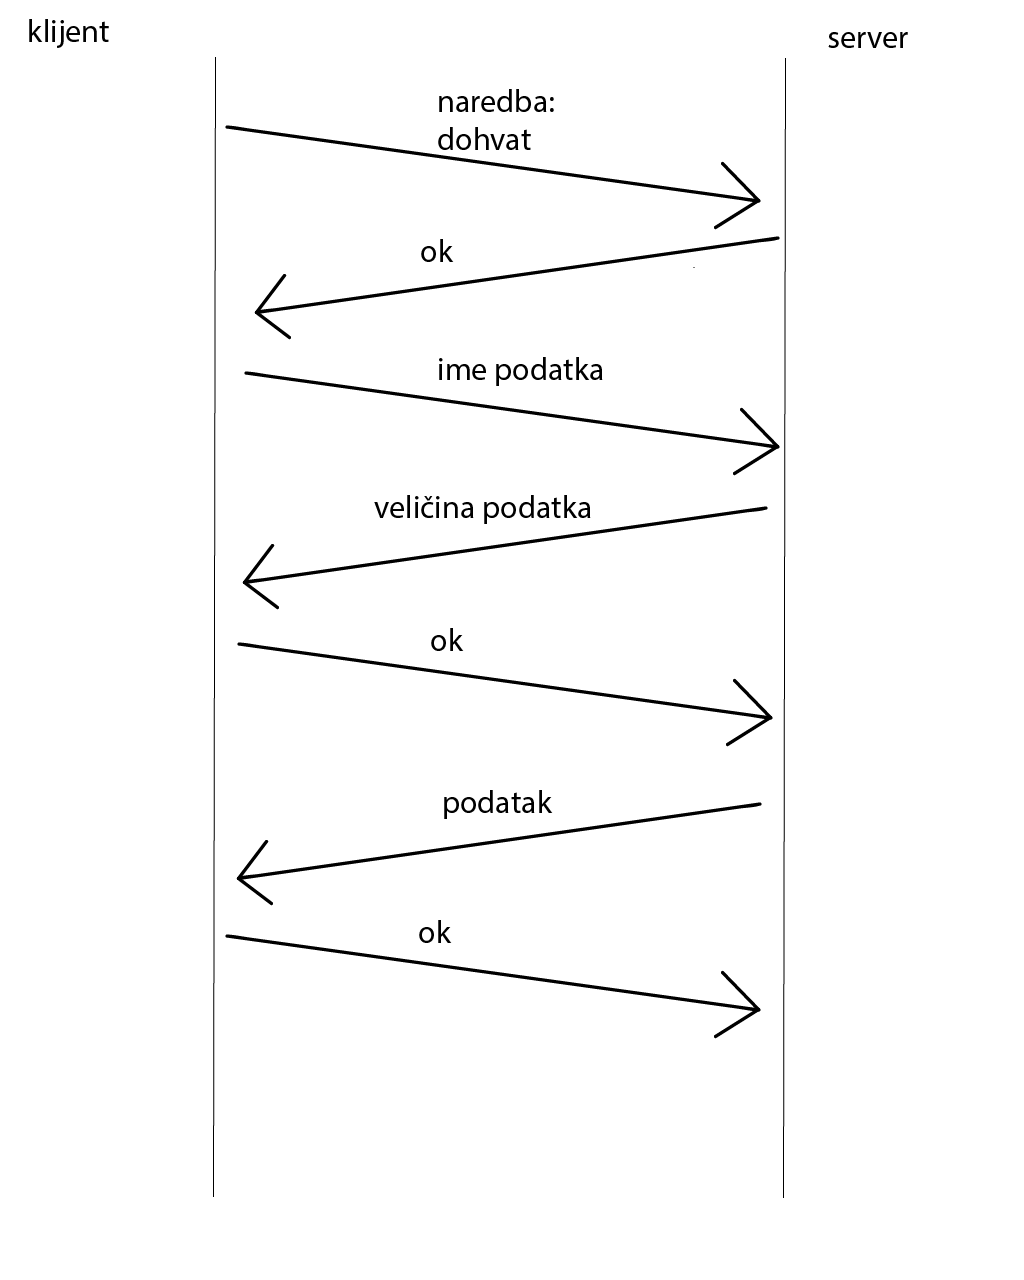
\includegraphics[width=0.5\textwidth]{graf_citanje_1}}}%
        \caption{Grafički prikaz protokola za čitanje i pisanje podataka na udaljeno računalo}
        \label{fig:graf_1}
    \end{figure}
    \FloatBarrier
\subsection{Rezultati}
Iz rezultata je vidljivo da ova implementacija pokazuje slabe rezultate pri razmjeni podataka s udaljenim računalom.
Očekivano je da će razmjena podataka s računalom na udaljenoj mreži biti sporija, ali čak i na lokalnoj mreži, vremena zapisa i čitanja s udaljenog računala pokazala su se dužima od razmjene podataka s trajnom memorijom.
Također iz grafa je vidljivo kako brzina razmjene podataka kod manjih podataka ne raste monotono u početku. Ono što se iz toga može zaključiti je da je protokol oko izmjene podataka usporio postupak pri manjim podacima.
Zanimljivo je da nema velike razlike u brzini prijenosa podataka s poslužiteljem neovisno o tome da li se klijent nalazi na računalu ili android uređaju.
Također je bitno primijetiti da kod android uređaja slabije raste vrijeme komunikacije s lokalnom memorijom nego kod ostalih datotečnih sustava, ali je zato kod manjih podataka sporiji od čvrstog diska i ssd memorije.
\begin{figure}[h!]
    \centering
    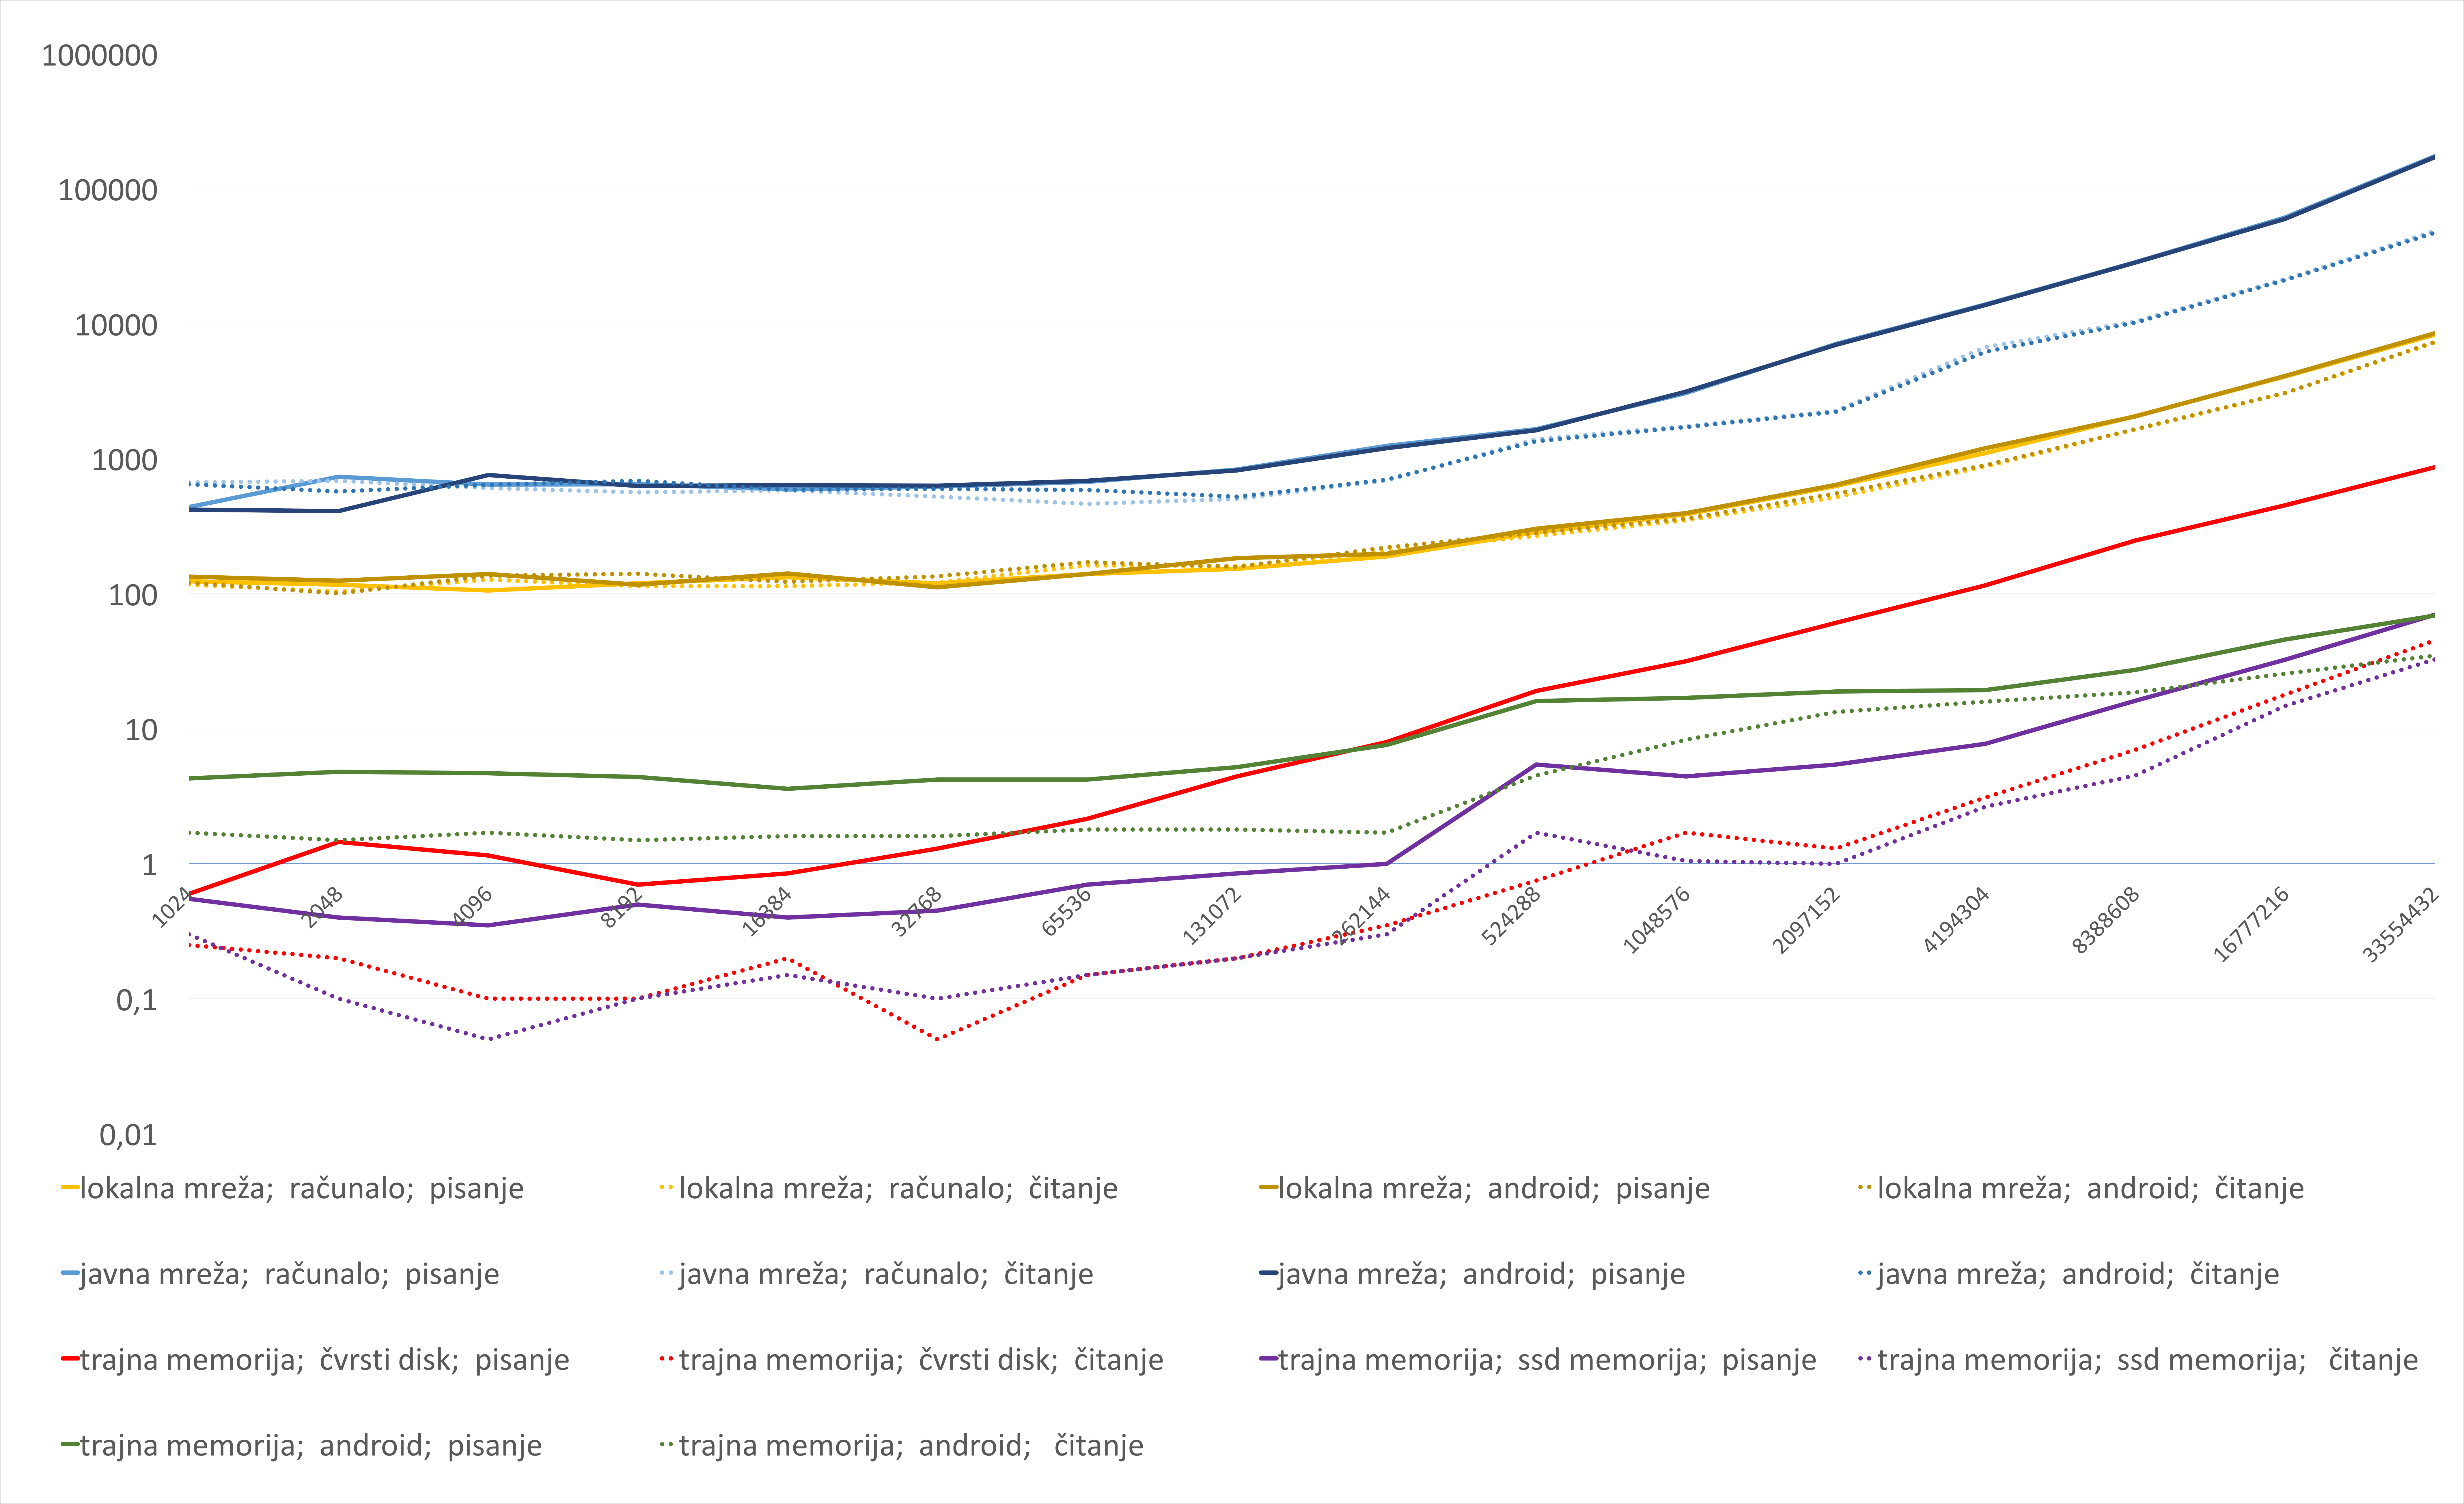
\includegraphics[width=1.5\textwidth, angle = 90]{1_graf}
    \caption{Brzine pisanja i čitanja svih stavki u sustavu sa strogim potvrđivanjem}
    \label{fig:rez_1}
\end{figure}
\FloatBarrier
\section{Sustav bez potvrđivanja}
Kako bi se smanjio utjecaj protokola na brzinu prijenosa podataka minimizirana je komunikacija s poslužiteljem prije i poslije izmjene podataka.
Podaci koji su nužni kako bi se mogao zapisati ili pročitati podatak su:

\begin{enumerate}
    \itemsep0em
    \item radnja koja se treba obaviti
    \item naziv podatka
    \item veličina podatka
\end{enumerate}

Kako se ne bi bilo potrebe za stalnom komunikacijom dodane su dvije klase, SocketMessageHelper i Header.
Klasa Header predstavlja zaglavlje koje se sastoji od navedenih podataka.
Header ima metodu koja ga pretvara u polje bajtova od 55 mjesta i ima konstruktor koji ga stvara iz polja bajtova.
SocketMessageHelper služi za standardiziranje informacija o operacijama.
U ovom sustavu je za zapis podataka na poslužitelj prije slanja samih podataka potrebno poslati samo zaglavlje nakon čega odmah počinje slanje podataka (Slika \ref{fig:graf_2}).
Kako bi se minimiziralo vrijeme komunikacije, ni u jednom trenutku se od poslužitelja ne traži potvrda da je slanje gotovo.
Za čitanje podataka od poslužitelja potrebno je dobiti informaciju o veličini podatka prije nego što se može započeti učitavati podatke, zbog čega čitanje u ovom slučaju ima jednu radnju više.
Nema promjena u komunikaciji s lokalnim datotečnim sustavom jer se već koriste jednostavne ugrađene operacije.
Jedini problem koji je nastao je taj da je kod nekih testiranja s podacima većim od 8MB došlo do pucanja veze zbog greške na slijedu podataka,
ali u većini testiranja se to nije dogodilo i zato su se uspješno skupili podaci o brzini slanja podataka.

\begin{figure}[h!]
    \centering
    \subfloat[zapis podataka]{{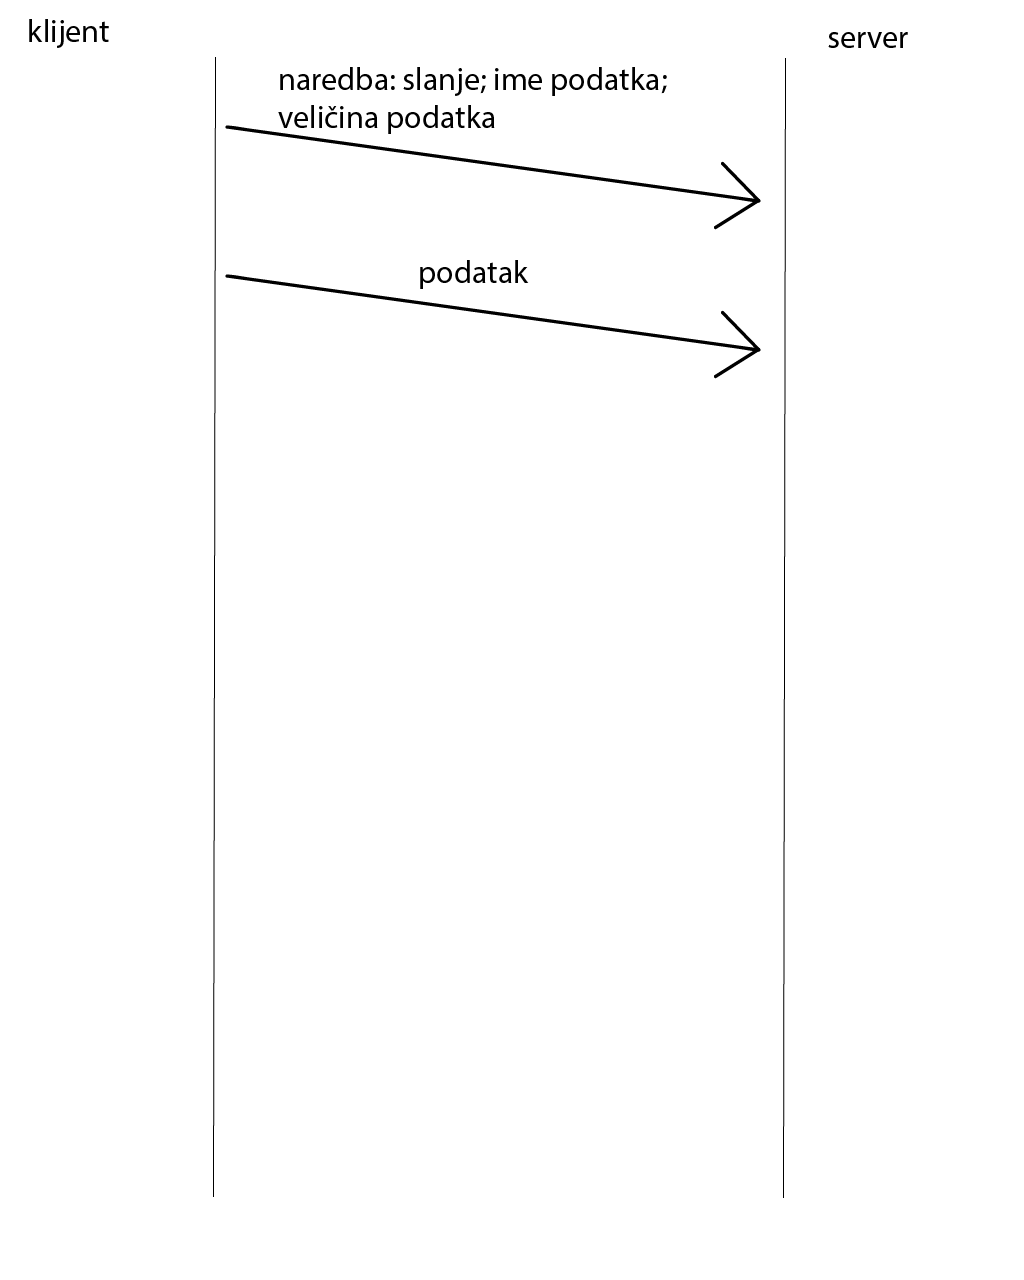
\includegraphics[width=0.5\textwidth]{graf_slanje_2}}}%
    \centering
    \subfloat[čitanje podataka]{{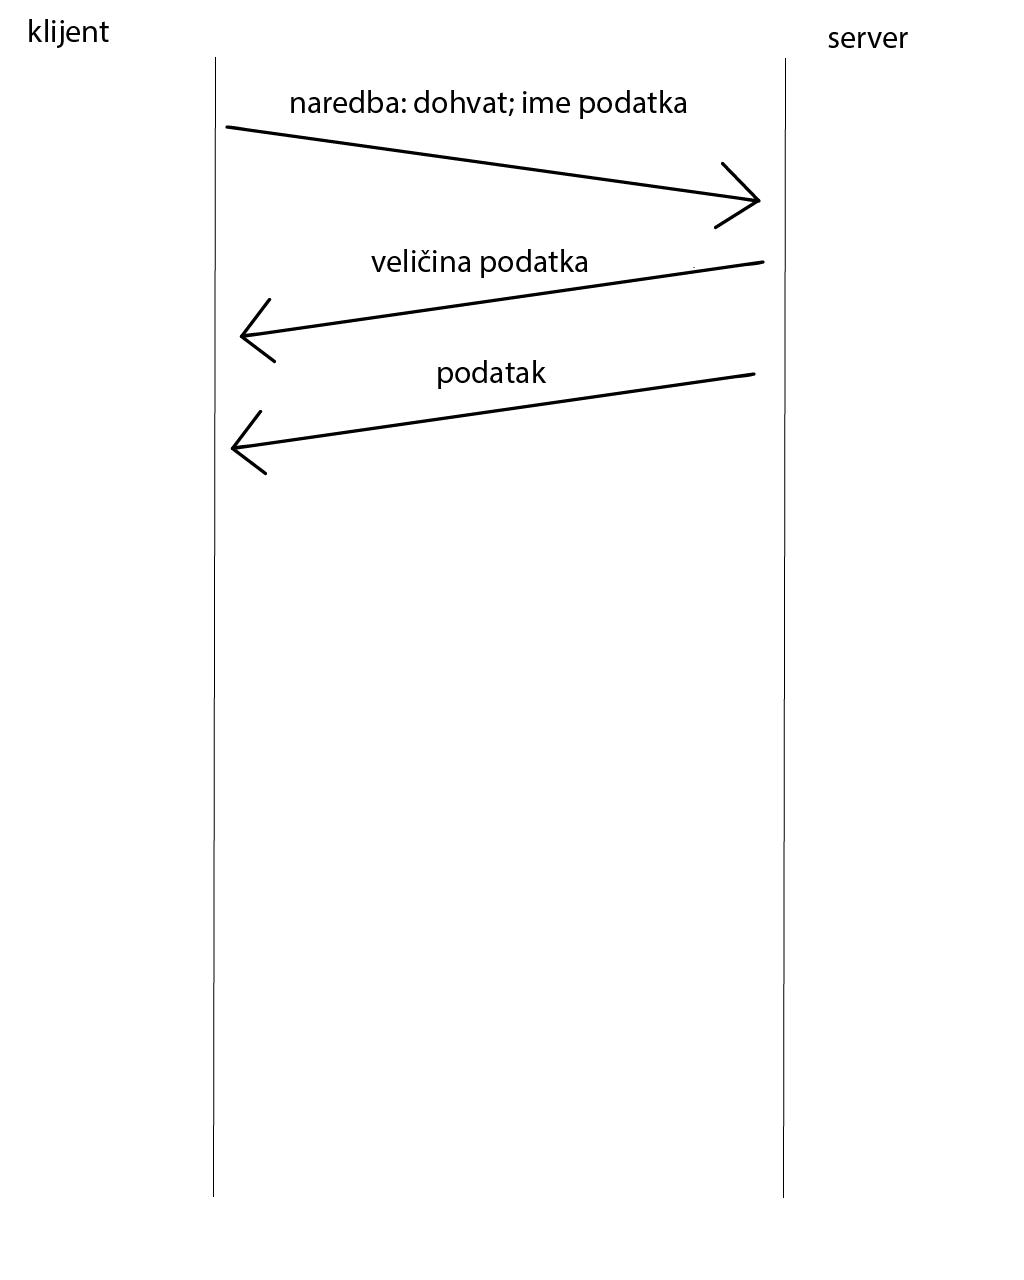
\includegraphics[width=0.5\textwidth]{graf_citanje_2}}}%
    \caption{Grafički prikaz protokola za čitanje i pisanje podataka na udaljeno računalo u sustavu bez potvrđivanja}
    \label{fig:graf_2}
\end{figure}

\subsection{Rezultati}
Ovom optimizacijom dobiveno je veliko smanjenje vremena potrebnog za izmjenu podataka s poslužiteljem kod manjih podataka.
Ono što je posebno interesantno je da se kod podataka manjih od 8kB pokazalo kako je zapisivanje podataka na udaljeno računalo 
brže od zapisivanja na čvrsti disk ili memoriju android uređaja, čak i kod javne mreže. 
Naravno ovdje se klijent ne brine o tome da li je poslužitelj učitao cijeli podatak prije nego krene sa sljedećom radnjom i ne znamo je li podatak uspješno spremljen na poslužitelju.
Takvih problema nema s čitanjem jer klijent zna da li je pročitao cijeli podatak.
Problem koji odmah možemo uočiti je to da kod zapisa većih podataka vrijeme raste u odnosu na prethodni test.
To se događa jer je ovaj sustav manje stabilan i opterećujemo izlazni slijed podataka bez da provjerimo je li poslužitelj sve uspio pročitati.
\begin{figure}[h!]
    \centering
    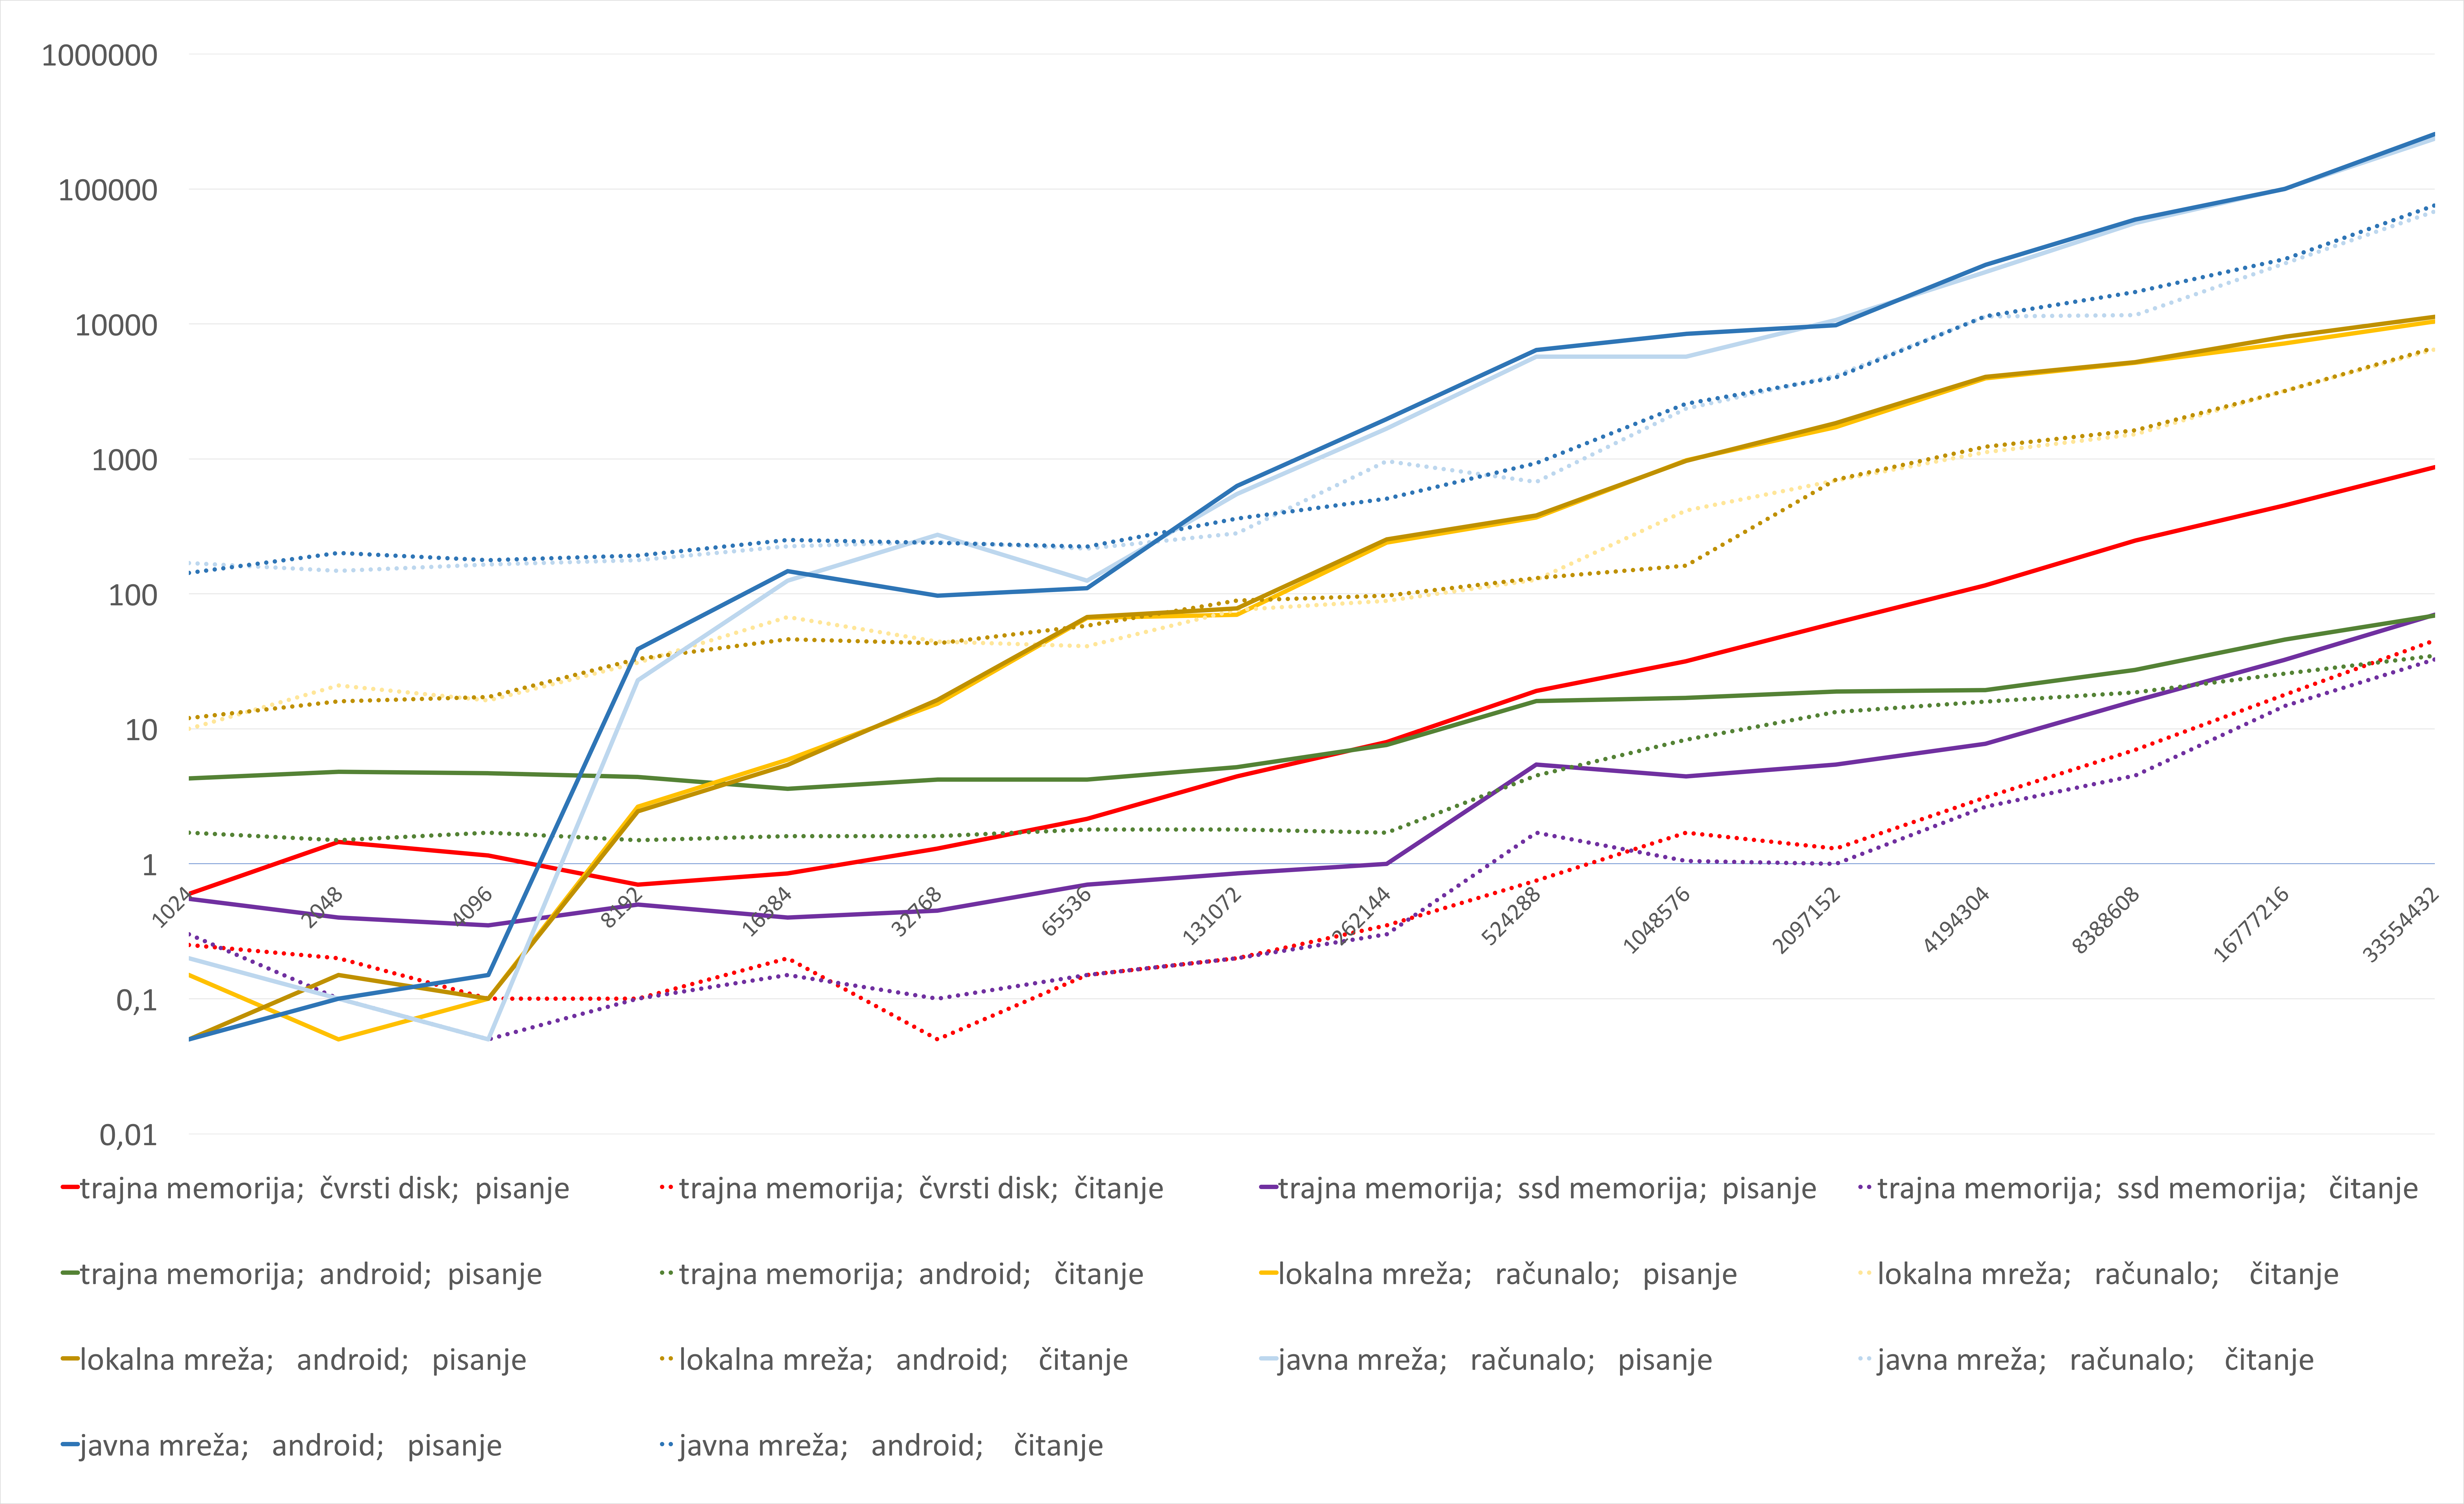
\includegraphics[width=1.5\textwidth, angle = 90]{2_graf}
    \caption{Brzine zapisa i čitanja svih stavki u sustavu bez potvrđivanja}
    \label{fig:graf}
\end{figure}
\begin{figure}[h!]
    \centering
    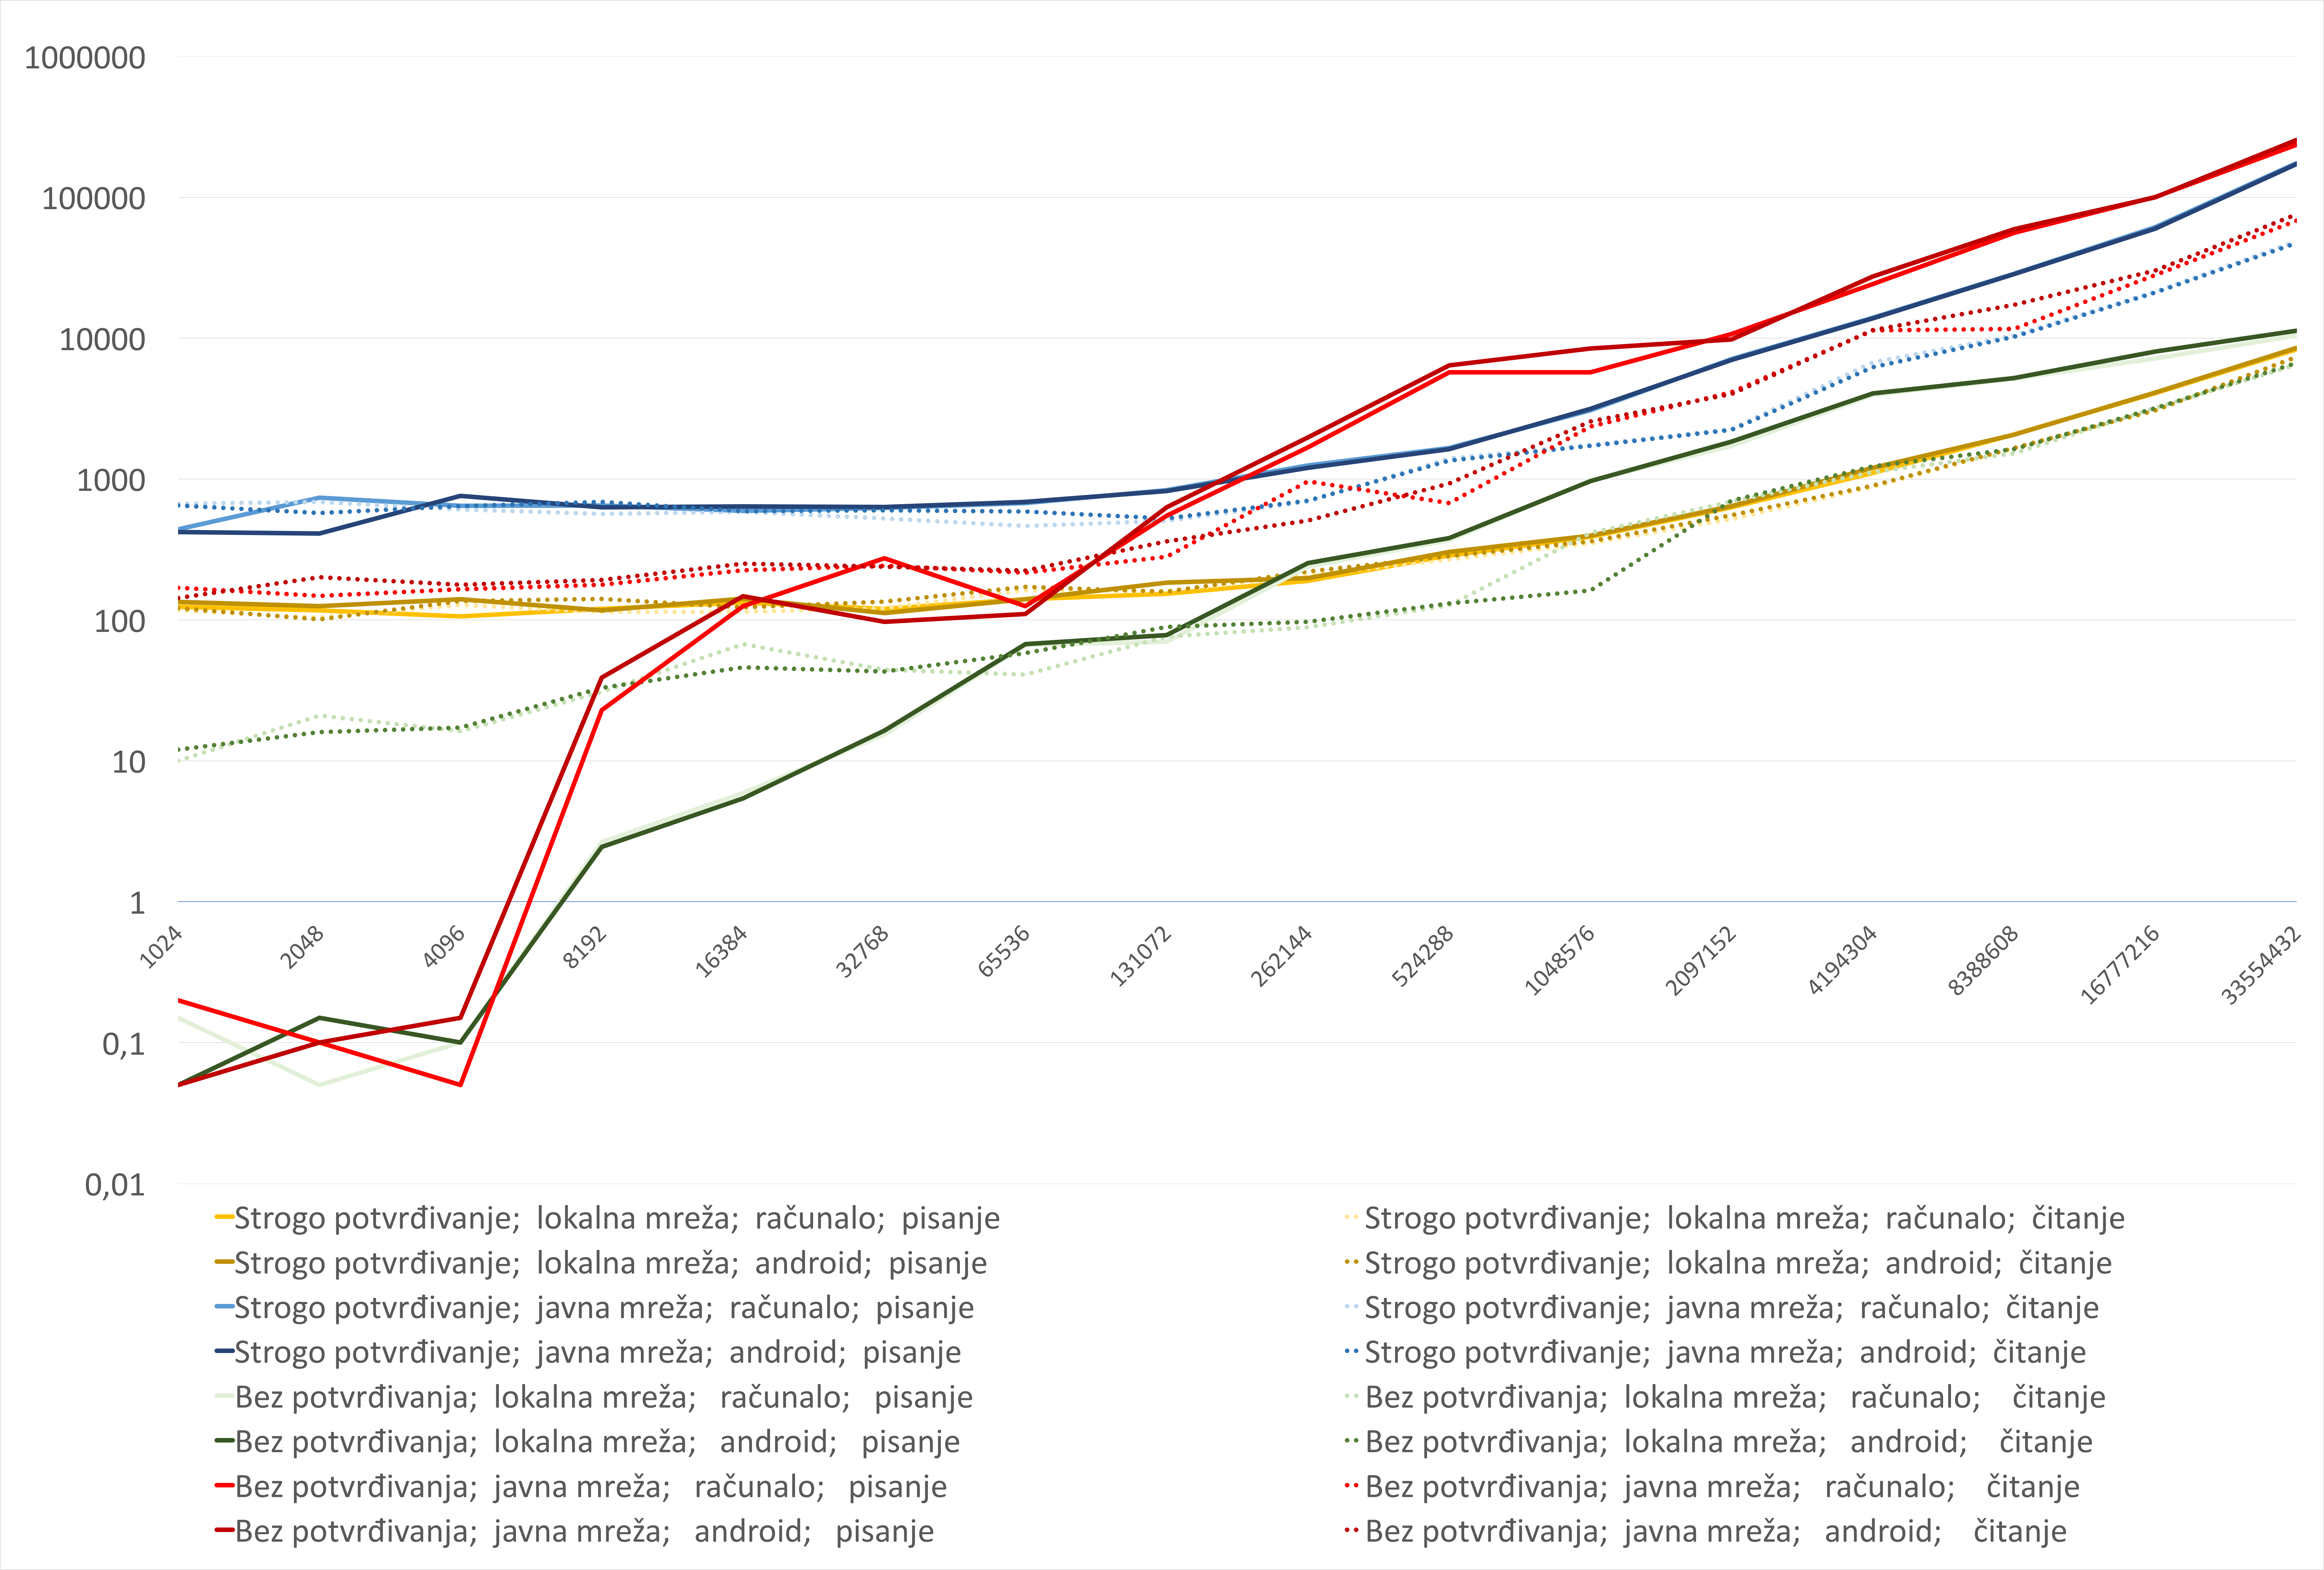
\includegraphics[width=1.5\textwidth, angle = 90]{2_1}
    \caption{Usporedba brzina sustava sa strogim potvrđivanjem i sustava bez potvrđivanja}
    \label{fig:graf_2_1}
\end{figure}
\FloatBarrier
\section{Sustav s minimalnim potvrđivanjem}
Kako bi se sa sigurnošću moglo reći da je podatak koji je potrebno spremiti na poslužitelj stvarno bio uspješno poslan, potrebna je povratna informacija od poslužitelja (Slika \ref{fig:graf_3}).
Naravno svaka dodatna izmjena podataka s poslužiteljem usporava ukupni postupak zapisivanja podataka. 
Jedna dodatna pozitivna stvar kod traženja povratne informacije na kraju slanja podataka na poslužitelj je ta što je osigurano da se neće slati novi podaci poslužitelju dok još nije pročitao posljednji podatak čime je dignuta stabilnost sustava.
Iz grafa na slici \ref{fig:graf_2_1} vidljivo je da je čitanje podataka s poslužitelja također pokazalo poboljšanje u zadnjem testu, a u toj operaciji postoji jedna operacija više\footnote{primanje veličine podatka od poslužitelja}, zato se može zaključiti da je prihvatljivo da klijent na kraju svakog zapisa od poslužitelja traži potvrdu da je prijenos gotov.

\begin{figure}[t]
    \centering
    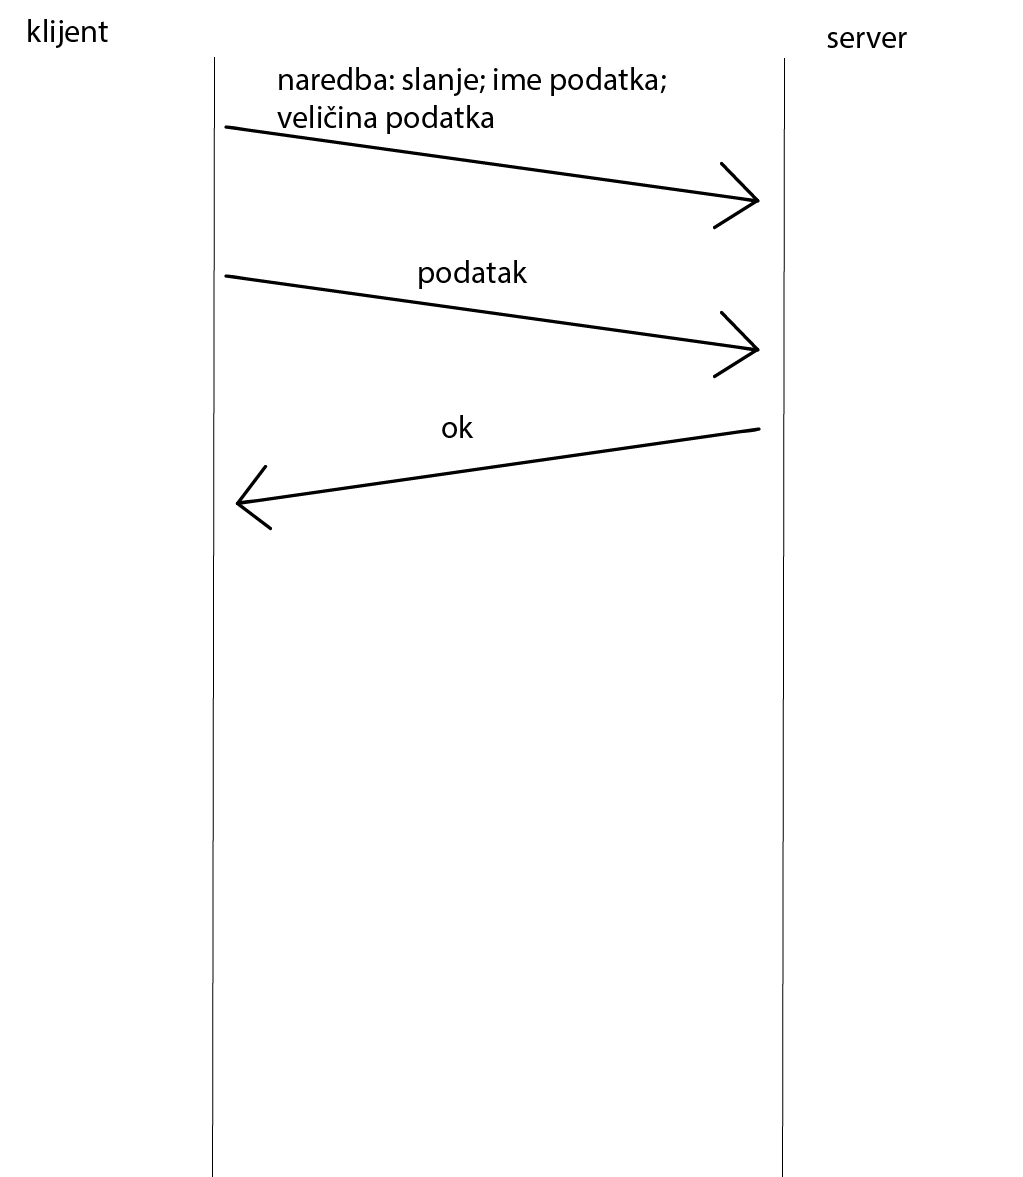
\includegraphics[width=0.5\textwidth]{graf_slanje_3}
    \caption{Grafički prikaz protokola s minimalnim potvrđivanjem}
    \label{fig:graf_3}
\end{figure}
\FloatBarrier
\subsection{Rezultati}
Kako je promjena bila samo u zapisivanju na poslužitelja, ne prikazuju se rezultati čitanja za ovaj test.
Vidljiv je rast u vremenu potrebnom da se završi postupak slanja manjih podataka u odnosu na test bez potvrđivanja.
Ono što je bitno za ovaj sustav je da je ovaj način stabilan, jednako brz kao prvi kod većih podataka, a puno brži od prvog testa kod manjih podataka.
Zapis podataka na lokalnoj mreži je kod malih podataka i dalje sličan brzini android memorije.

\begin{figure}[t]
    \centering
    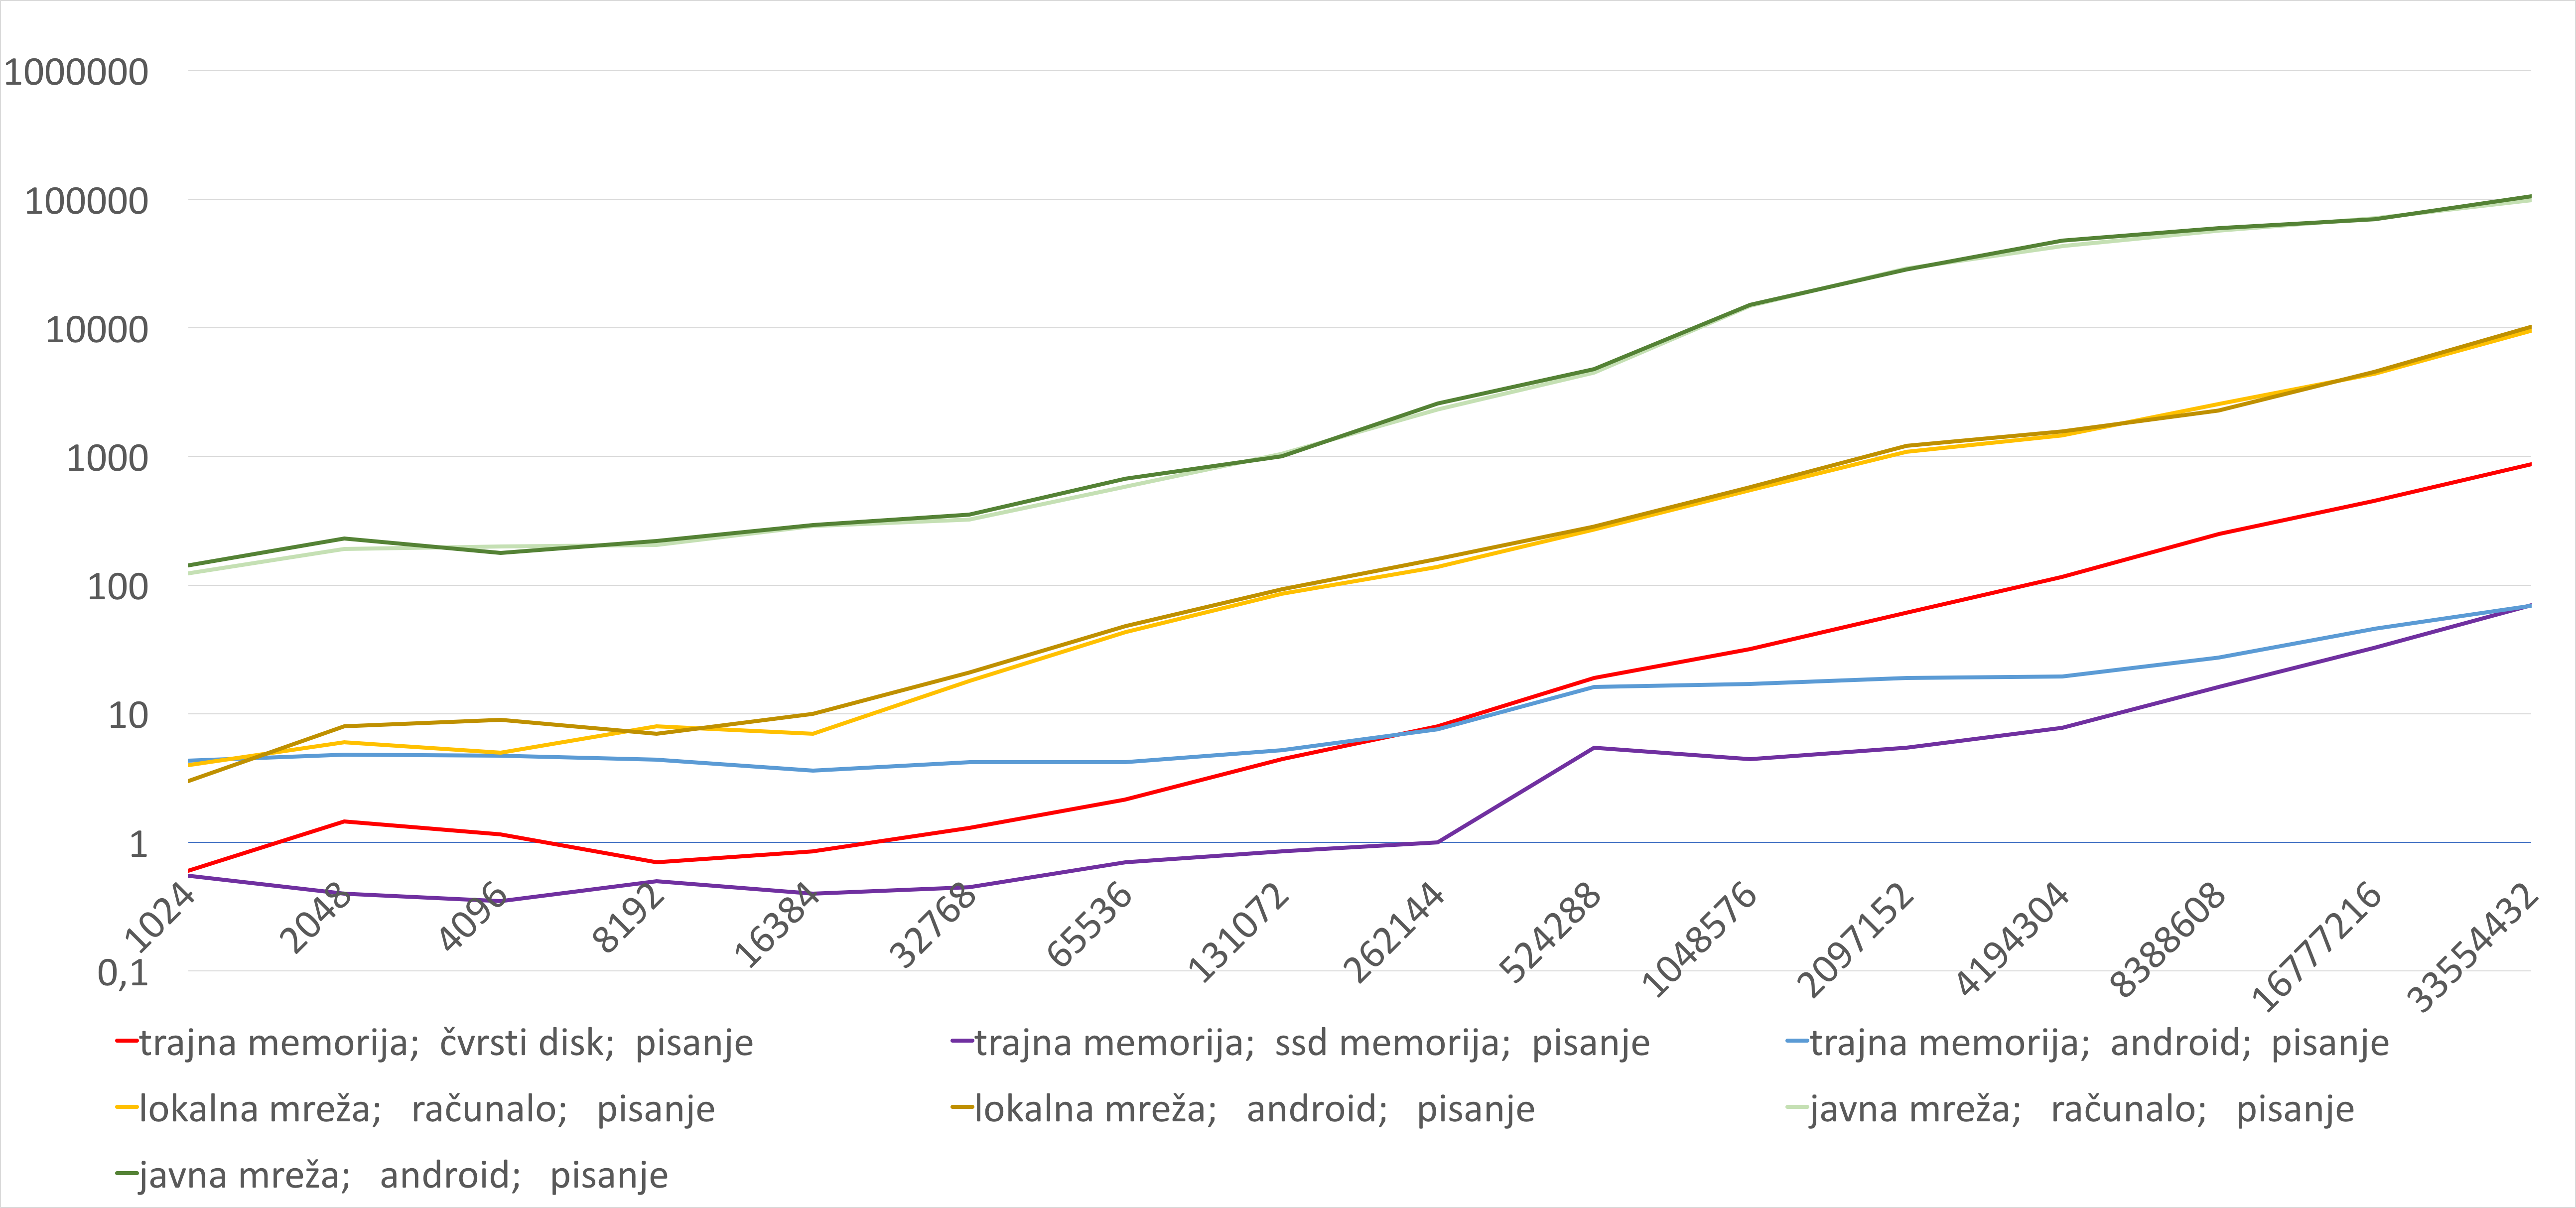
\includegraphics[width=1\textwidth]{3_graf}
    \caption{Usporedba brzine pisanja podataka sustava s minimalnim potvrđivanjem s lokalnim datotečnim sustavima}
    \label{fig:rez_1}
\end{figure}
\begin{figure}[t]
    \centering
    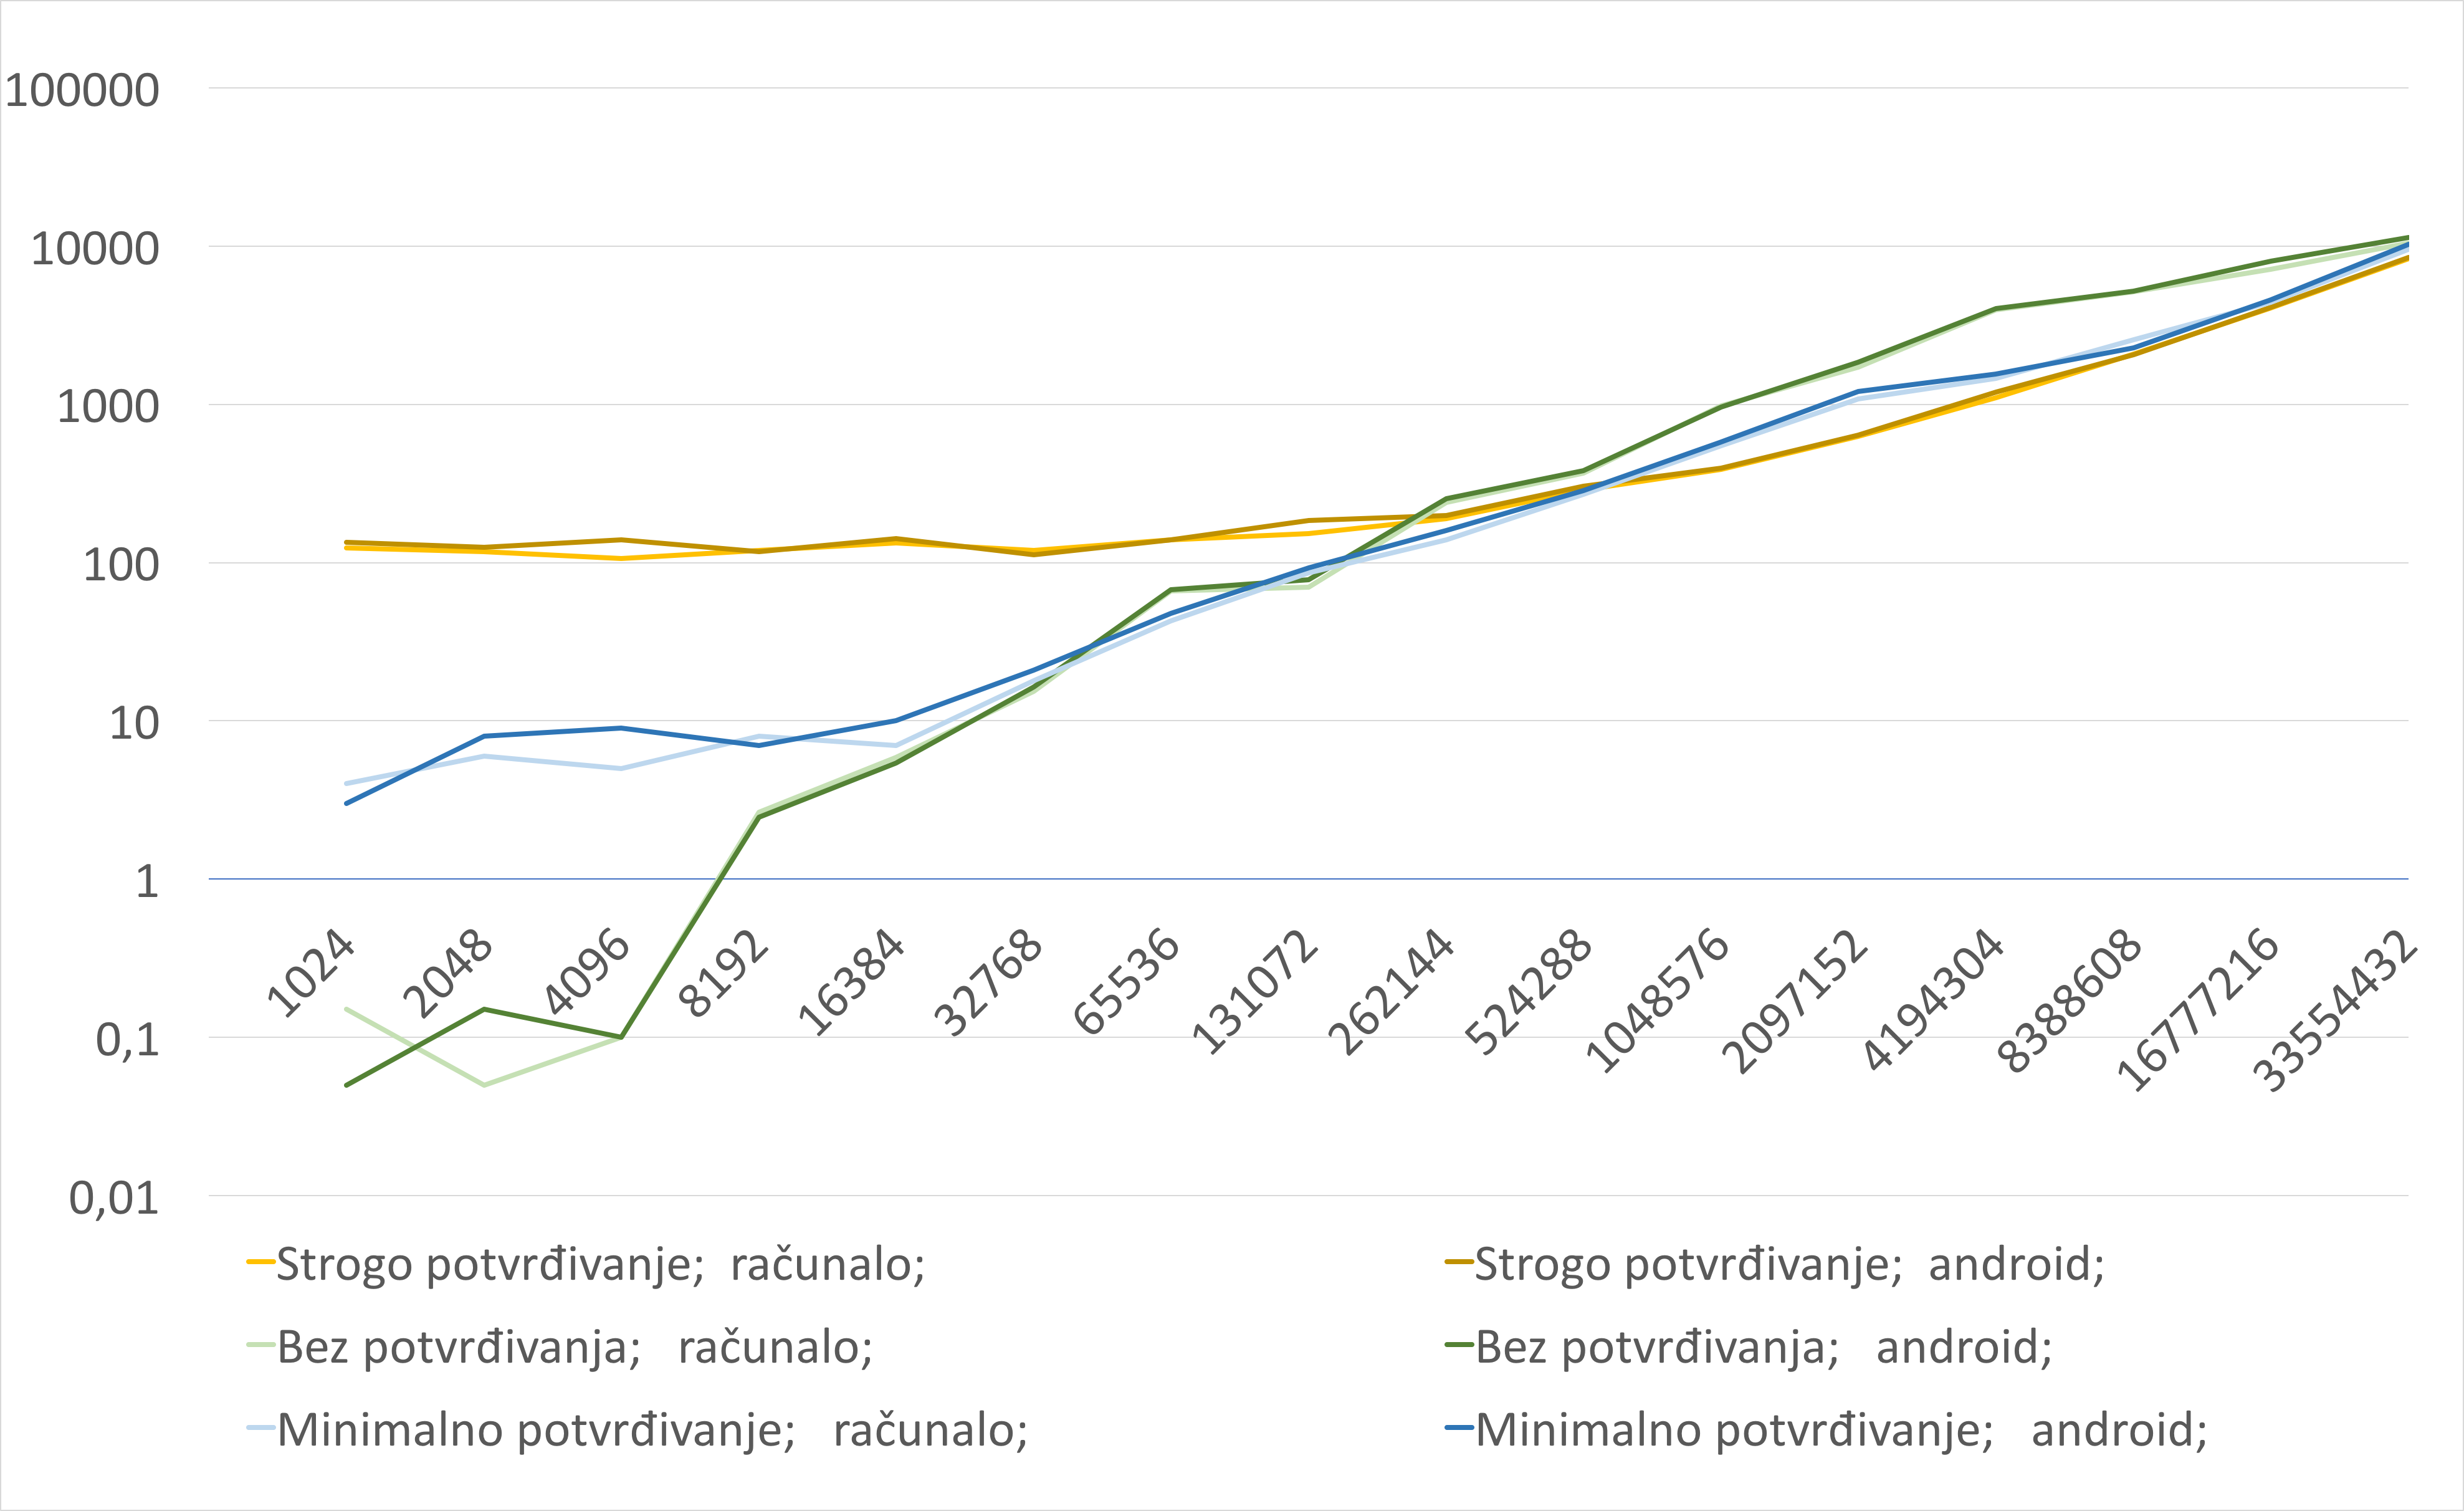
\includegraphics[width=1\textwidth]{3_2_1_lokalna}
    \caption{Usporedba svih testova u lokalnoj mreži}
    \label{fig:rez_1}
\end{figure}
\begin{figure}[t]
    \centering
    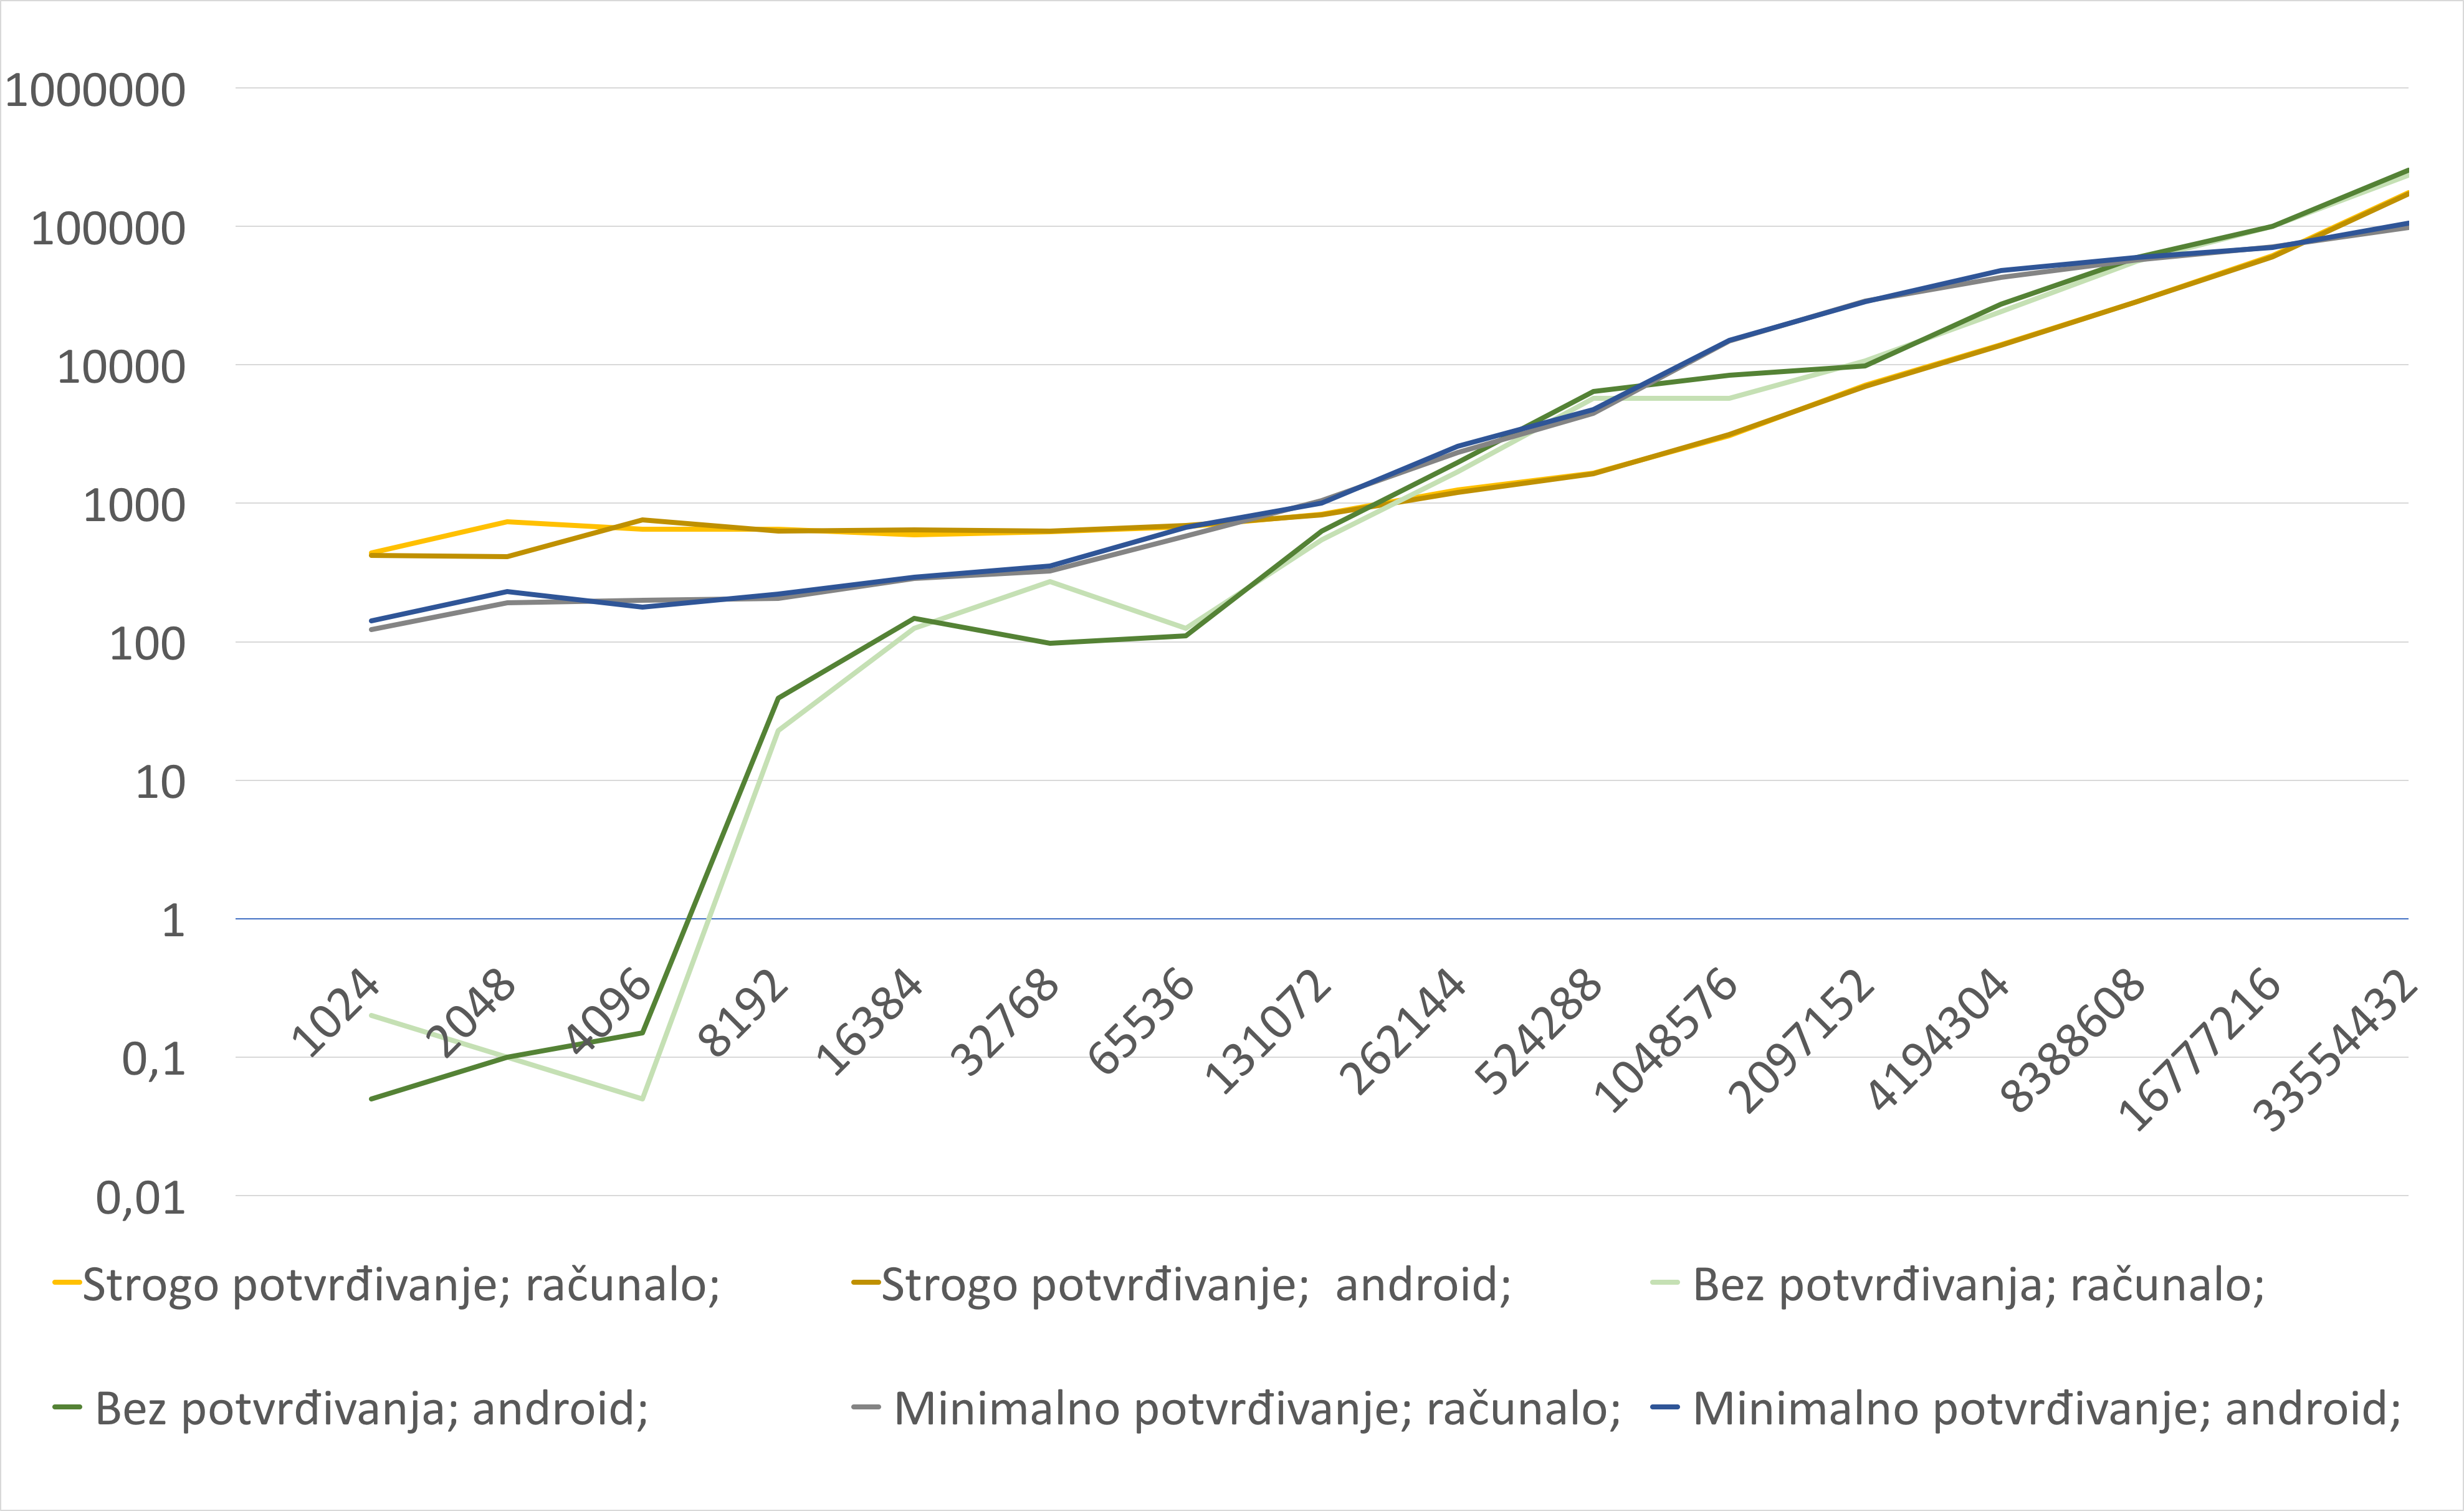
\includegraphics[width=1\textwidth]{3_2_1_javna}
    \caption{Usporedba svih testova u javnoj mreži}
    \label{fig:rez_1}
\end{figure}
\FloatBarrier
\section{Korištenje sustava}
Sustav se sastoji od poslužitelja i klijenta.
Poslužiteljska aplikacija se koristi tako da se ukuca broj port-a koji će se koristiti za spajanje na poslužiteljsku aplikaciju nakon čega je više nije potrebno imati interakciju s aplikacijom, primjer se može vidjeti na slici \ref{fig:server}.
Kod klijentske aplikacije u potrebno je upisati više podataka potrebnih za sve testove koji se izvode, kao što je vidljivo na slici \ref{fig:autoClient} to su redom:
    \begin{enumerate}
    \itemsep0em
    \item IP adresa poslužitelja
    \item pristupna točka poslužitelja
    \item naziv vrste trajne memorije koja će se koristiti
    \item lokacija na koju će se spremati testni podaci
    \item ime testa
    \item koristimo li sustav koji šalje podatke u zaglavlju (sustav bez potvrđivanja i sustav s minimalnim brojem potvrđivanja)
    \item ako je prethodan odgovor potvrdan, treba li server slati potvrdu kada pročita cijeli podatak
    \end{enumerate}
    \begin{figure}[t]
        \centering
        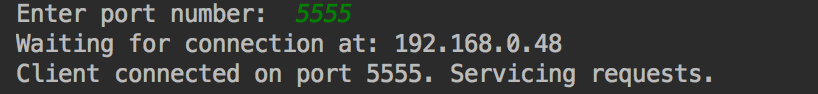
\includegraphics[width=1\textwidth]{server}
        \caption{prikaz terminala kod inicijalizacije poslužitelja }
        \label{fig:server}
    \end{figure}
    \begin{figure}[t]
        \centering
        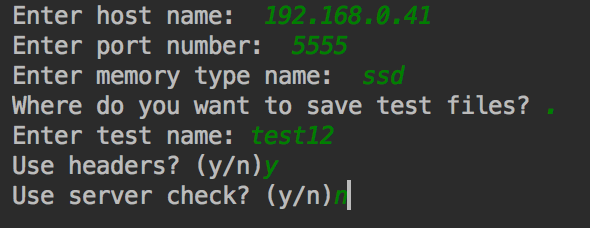
\includegraphics[width=0.8\textwidth]{autoClient}
        \caption{prikaz terminala prilikom upisa potrebnih podataka na klijentu}
        \label{fig:autoClient}
    \end{figure}
Nakon unosa navedenih podataka aplikacija će izvršiti testove i zapisati rezultate u csv (eng.\textit{ Comma Seperated Values}) datoteku.

Android aplikacija sastoji se od dva polja u koja se upisuju IP i port poslužitelja, gumba za pokretanje testova i prozora s informacijama, kao što je vidljivo na slici \ref{fig:android_ui}.
Za pokretanje testa unose se potrebni podaci i pritišće gumb koji odgovara testu koji se želi pokrenuti. 
Kada je test pokrenut odvijaju se jednake operacije kao kod klijenta na računalu.


   
\begin{figure}[h!]
    \centering
    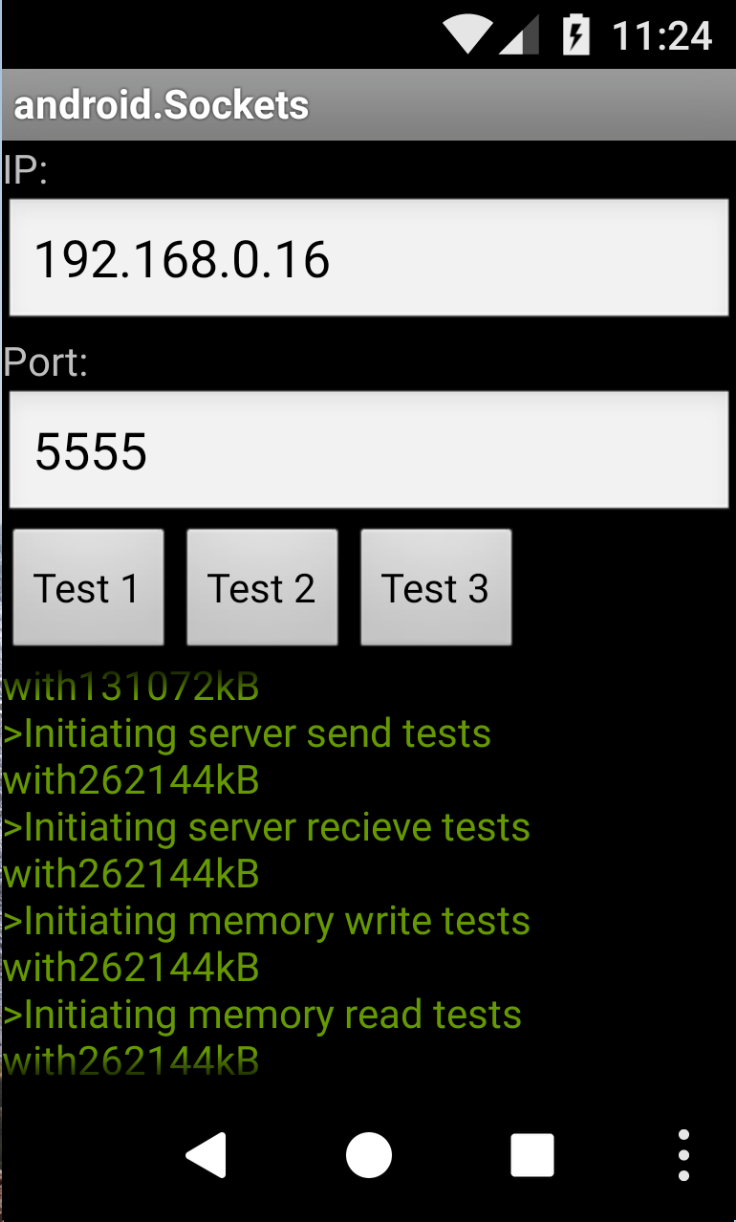
\includegraphics[width=0.5\textwidth]{android_ui}
    \caption{Zaslon android uređaja za vrijeme testa}
    \label{fig:android_ui}
\end{figure} 
\chapter{Zaključak}
U većini situacija zapisivanje i čitanje podataka brže je na trajnoj memoriji nego na radnu memoriju udaljenog računala.
Jedina situacija kada se pokazalo da je brže poslati podatke na udaljeno računalo je kada je potrebno spremiti jako mali podatak, a nije potrebna povratna informacija od poslužitelja da je zapis uspio.
Budući da kod malih podataka ne dolazi do pucanja veze s poslužiteljem, taj je pristup prihvatljiv ako je radnoj memoriji dovoljno držati samo manje podatke na drugoj memoriji.
Iako postoji situacija u kojoj se isplati slati podatke na udaljeno računalo, ta situacija nije dovoljno učestala da bi je opravdali kao standardnu operaciju, pogotovo jer je korištenje lokalnog datotečnog sustava jednostavnije i pouzdanije rješenje.
Jedino na android uređaju koji u pravilu imaju manju radnu memoriju i lokalnu memoriju, a zapis malih podataka na trajnu memoriju je relativno spor, ovakvo rješenje se isplati uzeti u obzir.
Naravno jednom kada su podaci poslani na udaljeno računalo, potrebno ih je i dohvatiti, a tu se udaljeno računalo uvijek pokazalo kao sporije od trajne memorije.


\bibliography{literatura}
\bibliographystyle{fer}

\begin{sazetak}
Glavne karakteristika radne memorije računala je ta da je brza, ali nije pogodna za trajno skladištenje podataka.
Zbog toga, ali i zato što je skupa, to je memorija manjeg kapaciteta od trajne memorije.
Ako lokalna radna memorija nema dovoljan kapacitet potrebno je podatke zapisati u trajnu memoriju ili poslati podatke na udaljeno računalo koje ih može čuvati spremne na svojoj radnoj memoriji.
Najveća prednost udaljene radne memorije je ta što su ti podaci spremni za pristup većem broju računala.
Nažalost pokazalo se kako je pristup podacima na radnoj memoriji udaljenog računala sporiji od pristupa na trajnoj memoriji, osim kod jako malih podataka kada nije potrebna potvrda od poslužitelja da su podaci uspješno pročitani.
Zbog toga, ako se ti podaci koriste samo za radnje pojedinog računala, najbolje je koristiti SSD memoriju koja je jednako brza kod manjih podataka, a puno brža kod velikih podataka.

\kljucnerijeci{čvrsti disk, hdd, ssd, ssd memorija, mrežna priključna točka, radna memorija}


\end{sazetak}
\pagebreak
% TODO: Navedite naslov na engleskom jeziku.
\engtitle{Performance Evaluation of Accessing Large Datasets Using Local File System and Remote RAM}
\begin{abstract}
Main characteristics of random access memory is that it is fast but not suitable for long term storage.
For that reason, and it's price, such memory is of lower capacity than non-volatile memory storage.
If local RAM doesn't have big enough capacity data must be stored in local memory or on remote device which can keep it ready in its random access memory.
The biggest advantage of remote random access memory is that it can be used by multiple devices.
Unfortunately it has been shown that data access to random access memory of remote computer is slower than accessing non-volatile memory, except with very small data when there is no need for server to confirm that data is successfully read.
For those reasons, if data is used only for single device, it is best to use solid-state drive which is just as fast with small data, and much faster with big data.

\keywords{hard disk, hdd, ssd, Solid State Drive, Socket, Network Socket, random access memory, ram}
\end{abstract}

\end{document}
